%\pdfoutput=1 %for arXiv submission
%\documentclass[iop,apj]{emulateapj}
\documentclass[twocolumn, twocolappendix]{aastex63}
\usepackage{hyperref}
\usepackage{amsmath,amstext}
\usepackage[T1]{fontenc}
%\usepackage{apjfonts} 
\usepackage{graphicx}
\usepackage[figure,figure*]{hypcap}
%\usepackage[fleqn]{amsmath}
\usepackage{multirow}
\usepackage{comment}
\usepackage{nicefrac}


\usepackage[]{algorithm2e} % algorithms


\renewcommand*{\sectionautorefname}{Section} %for \autoref
\renewcommand*{\subsectionautorefname}{Section} %for \autoref

%%% software mentioned again and again
\def\SPARK{\texttt{SPARK}}
\def\TARDIS{\texttt{TARDIS}}
\def\AUTOSTRUCTURE{\texttt{AUTOSTRUCTURE}}
\def\approxposterior{\texttt{approxposterior}}

%%% other useful commands
\def\citneeded{\textcolor{red}{\textbf{(citation needed)}}}
\newcommand\redbf[1]{\textbf{\textcolor{red}{#1}}}

\newcommand{\crf}[1]{{\color{violet} RF: #1}} %comment from Rodrigo
\usepackage{soul}
\newcommand{\remove}[1]{{\color{red} \st{#1}}}
\newcommand{\addtext}[1]{{\color{blue} #1}}

\def\lbol{${L}_{\rm bol}$}
\def\ledd{${L}_{\rm Edd}$}
\def\lsun{${L}_{\odot}$}
\def\sun{$_{\odot}$}
\def\lx{${L}_{\rm X}$}
\def\fx{${f}_{\rm X}$}
\def\f28{${f}_{2-8{\rm keV}}$}
\def\fr{${f}_R$}
\def\fo{f$_{opt}$}
\def\fxfr{${f}_X$/${f}_R$}
\def\fratio{${f}_X$/${f}_R$} 
\def\fxfopt{${f}_X$/${f}_{opt}$}
\def\fxfV{${f}_X$/${f}_V$}
\def\nh{N$_{\rm H}$}
\def\rc{r$_c$}
\def\mass{${\cal M}$}
\def\msun{${\cal M}_{\odot}$}
\def\mearth{${\cal M}_{\oplus}$}
\def\sun{$_{\odot}$}
\def\mdot{$\dot{\cal M}$}

\def\ergs{erg s$^{-1}$}
\def\ergscm2{erg s$^{-1}$ cm$^{-2}$}
\def\yr-1{yr$^{-1}$}
\def\kms{km s$^{-1}$}
\def\persec{\,\hbox{s}^{-1}}
\def\percc{\,\hbox{cm}^{-3}}
\def\persqcm{\,\hbox{cm}^{-2}}
\def\mic{\,\mu \hbox{m}}

\def\eg{{\it e.g.}}
\def\et{{\it et al.}}
\def\ie{{\it i.e.}}
\def\cf{{\it cf.}}

\def\a{$\&$}
\def\x{$\times$}
\def\about{$\sim$}
\def\simlt{\buildrel{<}\over \sim}
\def\simgt{\buildrel{>}\over \sim}
\def\simeq{\sim \over $=$}
\def\simgreat{\buildrel{>}\over \sim}
\def\simlt{$\la$}
\def\simgt{$\ga$}
\def\half{${\textstyle{1\over2}}$}
\def\thalf{{\textstyle{ 3\over 2}}}
\def\subr #1{_{{\rm #1}}}
\def\w{$\omega$}
\def\sig{$\sigma$}

\def\deg{$^{\rm o}$}
%\def\asec{$''$} 
\def\asec{\ifmmode^{\prime\prime}\else$^{\prime\prime}$\fi}
\def\amin{$'$}
\def\spt{$\buildrel{\prime\prime}\over .$}
\def\secspt{$\buildrel{\prime\prime}\over .$}
\def\minspt{$\buildrel{\prime}\over .$}
\def\magspt{$\buildrel{\rm m}\over .$}

%\def\Chandra{{\it Chandra}}
%\def\XMM{XMM {\it Newton}}
%\def\Rosat{{\it Rosat}}
%\def\Einstein{{\it Einstein}}
%\def\HST{{\it HST}}
%\def\Swift{{\it Swift}}
%\def\Nustar{{\it NuSTAR}}

\hypersetup{linkcolor=magenta}

\submitjournal{ApJ}
%\received{(ApJ) September 14, 2022}
%\accepted{on December 22, 2022}

\shorttitle{multi-component ejecta for the GW170817 kilonova} 
\shortauthors{Vieira {\it et al.}}

\begin{document}

\title{No Need for Multiple Components to fit the Spectra of the GW170817 Kilonova --- Spectroscopic $r$-Process Abundance Retrieval for Kilonovae II}

\correspondingauthor{Nicholas~Vieira}
\email{nicholas.vieira@mail.mcgill.ca}

\author[0000-0001-7815-7604]{Nicholas~Vieira}
\affil{Trottier Space Institute at McGill and Department of Physics, McGill University, 3600 rue University, Montreal, Qu{\'e}bec, H3A 2T8, Canada}

\author[0000-0001-8665-5523]{John~J.~Ruan}
\affil{Department of Physics and Astronomy, Bishop's University, 2600 rue College, Sherbrooke, Qu{\'e}bec, J1M 1Z7, Canada}

\author[0000-0001-6803-2138]{Daryl Haggard}
\affil{Trottier Space Institute at McGill and Department of Physics, McGill University, 3600 rue University, Montreal, Qu{\'e}bec, H3A 2T8, Canada}

\author[0000-0001-8921-3624]{Nicole Ford}
\affil{Trottier Space Institute at McGill and Department of Physics, McGill University, 3600 rue University, Montreal, Qu{\'e}bec, H3A 2T8, Canada}

% \author[0000-0001-7081-0082]{Maria~R.~Drout}
% \affil{Department of Astronomy and Astrophysics, University of Toronto, 50 St. George St., Toronto, Ontario, M5S 3H4, Canada}

% \author[0000-0003-4619-339X]{Rodrigo Fern{\'a}ndez}
% \affil{Department of Physics, University of Alberta, Edmonton, Alberta, T6G 2E1, Canada}

% \author{N.~R.~Badnell}
% \affil{Department of Physics, University of Strathclyde, Glasgow, G4 0NG, UK}



\begin{abstract}
x
\end{abstract}
\keywords{nuclear abundances, r-process, radiative transfer simulations, spectral line identification}

% ====================================================

%%% === SECTION 1 === %%%
%% INTRODUCTION %%
\section{Introduction}\label{sec:intro}

\begin{itemize}

    \item The $r$-process, its connection to neutron star mergers; connection to GW170817

    \item \SPARK~paper 1: technique, key results
    
    \item Single versus multi-component models of kilonova ejecta
    
    \item Goal of this paper: fit the later epochs to understand the time evolution of the abundances and determine whether multiple ejecta components are needed to fit the spectra
    
\end{itemize}

%%% === SECTION 2 === %%%
%% METHODS %%

\section{Methods}\label{sec:methods}

%%% SUBSECTION 2.1
\subsection{Spectroscopic $r$-Process Abundance Retrieval for Kilonovae (\textsc{SPARK})}\label{ssc:spark-summary}

We briefly describe our tool, Spectroscopic $r$-Process Abundance Retrieval for Kilonovae (\SPARK), and refer the reader to \cite{vieira23} for more detail. \SPARK is designed as a modular inference engine for extracting key parameters of kilonovae spectra, determining the element-by-element abundance pattern of the ejecta and associating features in the spectrum with particular species. 

In \SPARK, we couple the \TARDIS~(\citealt{kerzendorf14})~radiative transfer code to the approximate posterior estimation scheme of \approxposterior~(\citealt{fleming18,fleming20}). We generate a set of synthetic spectra, each parameterized by some $\theta_i$ including a luminosity, density, inner/outer computational boundary velocities, and three key parameters which determine the abundances in the ejecta: the electron fraction $Y_e$, expansion velocity $v_{\mathrm{exp}}$, and specific entropy per nucleon $s / k_{\mathrm{B}}$. These parameters describe different abundances from the nuclear reaction network calculations of \cite{wanajo18}. We write down a likelihood function using the full formalism of \cite{czekala15} for inference on spectroscopic data. Because of the considerable computational cost of spectral synthesis with \TARDIS, we do not use more common methods such as Markov chain Monte Carlo (MCMC) or nested sampling for inference---rather, we introduce a Gaussian Process (GP) surrogate for the posterior $L_p (\theta)$ and employ Bayesian Active Posterior Estimation (BAPE; \citealt{kandasamy17}). BAPE is a form of active learning in which we maximize an acquisition function with terms including both the mean $\mu(\theta)$ and variance $\sigma^2(\theta)$ of the GP. This acquisition function thus balances exploration (of the parameter space) and exploitation (sampling around the peak of the posterior). The GP is iteratively re-trained as new points $(\theta, L_p(\theta))$ are added to a training set and converges to an approximation of the posterior. 

The net result is that inference is dramatically accelerated, and we obtain (among the other kilonova parameters) the $Y_e$, $v_{\mathrm{exp}}$, $s / k_{\mathrm{B}}$ which best describe the ejecta with relatively few forward model evaluations. In \cite{vieira23}, we fit the VLT/X-shooter spectrum of the GW170817 kilonova at 1.4 days post-merger (\citealt{pian17, smartt17}) with a baseline of 1500 Latin Hypercube samples + 1140 BAPE active learning samples. This is a factor of $\sim 10^3$ fewer samples than might be required with a standard MCMC for a similar 6D fit.

%%% SUBECTION 2.2
\subsection{Multi-component, stratified ejecta with \textsc{TARDIS}}\label{ssc:multi-component-TARDIS}

\begin{itemize}

    \item Explain the single-component ejecta as used in the first paper

    \item In \cite{vieira23}, we model the kilonova ejecta as a single shell with a uniform abundance pattern. The plasma in this shell is also described by a single temperature and mass/electron density. This configuration is fully described by the luminosity at the outer boundary $L_{\mathrm{outer}}$, (which in fact sets the temperature at the inner boundary), the normalization in the density power law $\rho_0$, the inner and outer boundary velocities $v_{\mathrm{inner}}$ and outer bound

    \item Explain multi-component ejecta: different components with different abundances; stratification; multiple shells

    \item Describe the new physics which can be captured when doing multi-component (curtaining, re-processing...)

    \item Explain the physical meaning of a multi-component ejecta; connect to GRMHD simulations and explain why or why not an ejecta might be better described by multiple components

\end{itemize}



%%% SUBSECTION 2.3
\subsection{Inference setup}\label{ssc:inference-setup}

\begin{itemize}

    \item Describe any differences in the configuration, if any
    
    \item Explain why we fit for $v_{\mathrm{outer}}$ at these later epochs, whereas we kept it fixed in paper 1

    \item Describe priors at 2.4 and 3.4 days, compare with that of 1.4 days; motivate; point to Table~\ref{tab:priors-single}

    \item (IF APPLICABLE) Describe use of either masking or the \cite{czekala15} formalism for down-weighting the short wavelength portion of the spectrum in the fits to the 3.4 day spectrum

    \item Describe priors for multi-component fits; point to Table~\ref{tab:priors-multi}

\end{itemize}


\begin{deluxetable}{c|ccc}
\centering
\tablecaption{Priors for the parameters of the single-component fits at 1.4, 2.4, and 3.4 days. $v_{\mathrm{outer}}/c$ is fixed to $0.35$ in the 1.4 day fit (\citealt{vieira23}).}
\tablehead{parameter & 1.4 days & 2.4 days & 3.4 days}
\startdata\tablewidth{1.0\textwidth}
 \vspace{2pt}
$\log_{10}(L_\mathrm{outer}/L_{\odot})$ & $[7.6, 8.0]$ & $[7.2, 7.8]$ & TBD \\ 
$\log_{10}(\rho_0/\mathrm{g~cm^{-3}})$ & $[-16.0, -14.0]$ & same & same \\
$v_{\mathrm{inner}}/c$& $[0.250, 0.340]$ & $[0.100, 0.275]$ & TBD \\
$v_{\mathrm{outer}}/c$& - & $[0.280, 0.400]$ & TBD \\
$v_{\mathrm{exp}}/c$ & $[0.05, 0.30]$ & same & same \\
$Y_e$ & $[0.01, 0.40]$ & same & same \\
$s~[k_{\mathrm{B}}/\mathrm{nucleon}]$ & $[10, 35]$ & same & same \\
\enddata
\end{deluxetable}\label{tab:priors-single}


\begin{deluxetable}{c|c}
\centering
\tablecaption{Priors for the parameters of the multi-component fits at 1.4, 2.4, and 3.4 days.}
\tablehead{parameter & prior}
\startdata\tablewidth{1.0\textwidth}
 \vspace{2pt}
$\log_{10}(L_\mathrm{outer}/L_{\odot})$ & $[7.5, 8.0]$ \\ 
$\log_{10}(\rho_0/\mathrm{g~cm^{-3}})$ & $[-16.0, -14.0]$ \\\hline
$v_{\mathrm{inner,red}}/c$& $[0.10, 0.35]$ \\
$v_{\mathrm{outer,red}}/c$ &  $[0.25, 0.40]$ \\
$v_{\mathrm{exp,red}}/c$ & $[0.05, 0.30]$ \\
$Y_{e,\mathrm{red}}$ & $[0.01, 0.45]$ \\
$s_{\mathrm{red}}~[k_{\mathrm{B}}/\mathrm{nucleon}]$ & $[10, 35]$ \\\hline
$v_{\mathrm{inner,blu}}/c$& $[0.10, 0.35]$ \\
$v_{\mathrm{outer,blu}}/c$ &  $[0.25, 0.40]$ \\
$v_{\mathrm{exp,blu}}/c$ & $[0.05, 0.30]$ \\
$Y_{e,\mathrm{blu}}$ & $[0.05, 0.50]$ \\
$s_{\mathrm{blu}}~[k_{\mathrm{B}}/\mathrm{nucleon}]$ & $[10, 35]$ \\
\enddata
\end{deluxetable}\label{tab:priors-multi}


%%% === SECTION 3 === %%%
%% RESULTS %%

\section{Results}\label{sec:results}

%%% === SECTION 4 === %%%
%% DISCUSSION %%

\section{Discussion}\label{sec:disco}

\subsection{Time evolution of the abundances}

\subsection{Single- versus multi-component}


%%% === SECTION 5 === %%%
%% CONCLUSIONS %%

\section{Conclusions}\label{sec:conclusions}



%%% === ACKNOWLEDGEMENTS === %%%
\acknowledgments


NV works in Tiohti{\'a}:ke / Mooniyang, also known as Montr{\'e}al, which lies on the unceded land of the Haudenosaunee and Anishinaabeg nations. This work made use of high-performance computing resources in Tiohti{\'a}:ke / Mooniyang and in Burnaby, British Columbia, the unceded land of the Coast Salish peoples, including the Tsleil-Waututh, Kwikwetlem, Squamish, and Musqueam nations. We acknowledge the ongoing struggle of Indigenous peoples on this land, and elsewhere on Turtle Island, and hope for a future marked by true reconciliation. 

This work made extensive use of the \href{https://docs.alliancecan.ca/wiki/Cedar}{\texttt{Cedar}} and \href{https://docs.alliancecan.ca/wiki/Narval/en}{\texttt{Narval}} clusters of the \href{https://alliancecan.ca/en}{Digital Research Alliance of Canada} at Simon Fraser University (with regional partner \href{https://www.westgrid.ca/}{WestGrid}) and the {\'E}cole de technologie sup{\'e}rieure, respectively. We thank the support staff of Calcul Qu{\'e}bec in particular for their assistance at various steps in this project. We also thank Nikolas Provatas, Victor Ionescu, and Bart Odelman.

We thank Shinya Wanajo for kindly sharing their reaction network calculations. We thank Jessica Birky and David Fleming for useful discussions on approximate Bayesian inference and the use of \href{https://dflemin3.github.io/approxposterior/index.html}{\approxposterior}.

This work has made use of the \href{http://vald.astro.uu.se/~vald/php/vald.php}{Vienna Atomic Line Database (VALD)}, operated at Uppsala University, the Institute of Astronomy RAS in Moscow, and the University of Vienna. We thank Nikolai Piskunov and Eric Stempels for help in obtaining the VALD data.

This research made use of \href{https://tardis-sn.github.io/tardis/index.html}{\TARDIS}, a community-developed software package for spectral synthesis in supernovae (\citealt{kerzendorf14}). The development of \TARDIS~received support from the Google Summer of Code initiative and from the European Space Agency (ESA)'s Summer of Code in Space program. \TARDIS~makes extensive use of \href{https://docs.astropy.org/en/stable/}{\texttt{astropy}}. We thank Andrew Fullard, Wolfgang Kerzendorf, and the entire \TARDIS~development team for their assistance and their commitment to the development and maintenance of the code. 

N.V. acknowledges funding from the Bob Wares Science Innovation Prospectors Fund and the Murata Family Fellowship. J.J.R.\ and D.H.\ acknowledge support from the Canada Research Chairs (CRC) program, the NSERC Discovery Grant program, the FRQNT Nouveaux Chercheurs Grant program, and the Canadian Institute for Advanced Research (CIFAR). J.J.R.\ acknowledges funding from the Canada Foundation for Innovation (CFI), and the Qu\'{e}bec Ministère de l’\'{E}conomie et de l’Innovation.
\newline

%%% === SOFTWARE === %%%
\software{
\href{https://dflemin3.github.io/approxposterior/index.html}{\approxposterior}: \cite{fleming18};
\href{https://docs.astropy.org/en/stable/}{\texttt{astropy}}: \cite{astropy18};
\href{https://cmasher.readthedocs.io/}{\texttt{cmasher}}: \cite{velden20};
\href{https://corner.readthedocs.io/en/latest/index.html}{\texttt{corner}}: \cite{foreman-mackey16};
\href{https://dynesty.readthedocs.io/en/latest/index.html}{\texttt{dynesty}}: 
\cite{speagle20};
% \href{https://emcee.readthedocs.io/en/stable/}{\texttt{emcee}}: \cite{foreman-mackey13}; 
\href{https://george.readthedocs.io/en/latest/}{\texttt{george}}: \cite{ambikasaran15};
\href{https://tardis-sn.github.io/tardis/index.html}{\TARDIS}: \cite{kerzendorf14};
% \href{https://johannesbuchner.github.io/UltraNest/}{\texttt{UltraNest}}: \cite{buchner21}
} 

\clearpage




%%% === BIBLIOGRAPHY === %%%
\bibliographystyle{apj}
\begin{thebibliography}{}


%\bibitem[Abbott \& Lucy(1985)]{abbott85} Abbott, D.~C. \& Lucy, L.~B.\ 1985, \apj, 288, 679
%%%%% TARDIS LUCY FORMALISM


% \bibitem[Abbott et al.(2017a)]{abbottLIGO17a} Abbott, B.~P., Abbott, R., Abbott, T.~D., et al.\ 2017a, \aj, 848, L12
% %%%%% G170817: MULTI-MESSENGER


% \bibitem[Abbott et al.(2017b)]{abbottLIGO17b} Abbott, B.~P., Abbott, R., Abbott, T.~D., et al.\ 2017b, \apjl, 848, L13
% %%%%% GW170817: GWs AND GRBs


% \bibitem[Abbott et al.(2017)]{abbott17c} Abbott, B.~P., Abbott, R., Abbott, T.~D., et al.\ 2017, \prl, 119, 161101
% %%%%% GW170817: GWs 

%\bibitem[Abbott et al.(2018)]{abbottLIGO18} Abbott, B.~P., Abbott, R., Abbott, T.~D., et al.\ 2018, Living Reviews in Relativity, 21, 3


%\bibitem[Abbott et al.(2018)]{abbott18} Abbott, T.~M.~C., Abdalla, F.~B., Allam, S., et al.\ 2018, \apjs, 239, 18


% \bibitem[Ai et al.(2022)]{ai22} Ai, S., Zhang, B., \& Zhu, Z.\ 2022, \mnras, 516, 2614


% \bibitem[Almualla et al.(2021)]{almualla21} Almualla, M., Ning, Y., Bulla, M., et al.\ 2021, arXiv:2112.1547
% %%%%% INFERENCE WITH POSSIS



\bibitem[Ambikasaran et al.(2015)]{ambikasaran15} Ambikasaran, S., Foreman-Mackey, D., Greengard, L., et al.\ 2015, IEEE Transactions on Pattern Analysis and Machine Intelligence, 38, 252


% \bibitem[Anand et al.(2021)]{anand21} Anand, S., Coughlin, M.~W., Kasliwal, M.~M., et al.\ 2021, Nature Astronomy, 5, 46
% %%%%% POSSIS DATASET USED IN LUKOSIUTE+22


% \bibitem[Andreoni et al.(2017)]{andreoni17} Andreoni, I., Ackley, K., Cooke, J., et al.\ 2017, \pasa, 34, e069
% %%%%% GW170817 OBSERVATIONS


% \bibitem[Arcavi et al.(2017)]{arcavi17} Arcavi, I., Hosseinzadeh, G., Howell, D.~A., et al.\ 2017, \nat, 551, 64
% %%%%% GW170817 OBSERVATIONS


%\bibitem[Arnett(1982)]{arnett82} Arnett, W.~D.\ 1982, \apj, 253, 785


\bibitem[Astropy Collaboration et al.(2018)]{astropy18} Astropy Collaboration, Price-Whelan, A.~M., Sip{\H{o}}cz, B.~M., et al.\ 2018, \aj, 156, 123


% \bibitem[Badnell(2016)]{badnell16} Badnell, N.~R.\ 2016, AUTOSTRUCTURE: General program for calculation of atomic and ionic properties, ascl:1612.014


% \bibitem[Baiotti \& Rezzolla(2017)]{baiotti17} Baiotti, L. \& Rezzolla, L.\ 2017, Reports on Progress in Physics, 80, 096901.


%\bibitem[Banerjee et al.(2020)]{banerjee20} Banerjee, P., Wu, M.-R., \& Yuan, Z.\ 2020, \apjl, 902, L34
%%%%% ASTROPHYSICAL SITE OF THE R-PROCESS


%\bibitem[Bar-Shalom et al.(2001)]{barshalom01} Bar-Shalom, A., Klapisch, M., \& Oreg, J.\ 2001, \jqsrt, 71, 169


%\bibitem[Barnes \& Kasen(2013)]{barnes13} Barnes, J., Kasen, D.\ 2013, \aj, 775, 18


% \bibitem[Barnes et al.(2016)]{barnes16} Barnes, J., Kasen, D., Wu, M., Mart\'{i}nez-Pinedo, G.\ 2016, \apj, 829, 110


% \bibitem[Barnes et al.(2021)]{barnes21} Barnes, J., Zhu, Y.~L., Lund, K.~A., et al.\ 2021, \apj, 918, 44


%\bibitem[Barstow \& Heng(2020)]{barstow20} Barstow, J.~K., \& Heng, K.\ 2020, arXiv e-prints, arXiv:2003.14311


% \bibitem[Bartos \& Marka(2019)]{bartos19} Bartos, I. \& Marka, S.\ 2019, \nat, 569, 85
% %%%%% ASTROPHYSICAL SITE OF THE R-PROCESS


% \bibitem[Bauswein et al.(2013)]{bauswein13} Bauswein, A., Goriely, S., \& Janka, H.-T.\ 2013, \apj, 773, 78



% \bibitem[Beniamini et al.(2016)]{beniamini16} Beniamini, P., Hotokezaka, K., \& Piran, T.\ 2016, \apj, 832, 149
% %%%%% ASTROPHYSICAL SITE OF THE R-PROCESS


%\bibitem[Bethe \& Brown(1998)]{bethe98} Bethe, H.~A., \& Brown, G.~E.\ 1998, \apj, 506, 780

% \bibitem[Bisterzo et al.(2014)]{bisterzo14} Bisterzo, S., Travaglio, C., Gallino, R., et al.\ 2014, \apj, 787, 10


% \bibitem[Brauer et al.(2020)]{brauer20} Brauer, K., Ji, A.~P., Drout, M.~R., et al.\ 2020, arXiv:2010.15837
% %%%%% ASTROPHYSICAL SITE OF THE R-PROCESS


% \bibitem[Buchner(2021)]{buchner21} Buchner, J.\ 2021, The Journal of Open Source Software, 6, 3001
% %%%%% ULTRANEST


% \bibitem[Bulla(2019)]{bulla19} Bulla, M.\ 2019, \mnras, 489, 5037


% \bibitem[Burbidge et al.(1957)]{burbidge57} Burbidge, E.~M., Burbidge, G.~R., Fowler, W.~A., et al.\ 1957, Reviews of Modern Physics, 29, 547


% \bibitem[Cameron(1957)]{cameron57} Cameron, A.~G.~W.\ 1957, \pasp, 69, 201


%\bibitem[Castor(1974)]{castor74} Castor, J.~L.\ 1974, \mnras, 169, 279
%%%%% EXPANSION OPACITY FORMALISM


% \bibitem[Chornock et al.(2017)]{chornock17} Chornock, R., Berger, E., Kasen, D., et al.\ 2017, \apjl, 848, L19


%\bibitem[Christie et al.(2019)]{christie19} Christie, I.~M., Lalakos, A., Tchekhovskoy, A., et al.\ 2019, \mnras, 490, 4811


% \bibitem[Ciolfi(2020)]{ciolfi20a} Ciolfi, R.\ 2020, General Relativity and Gravitation, 52, 59
% %%%%% IMPORTANCE OF B-FIELDS


% \bibitem[Ciolfi \& Kalinani(2020)]{ciolfi20b} Ciolfi, R. \& Kalinani, J.~V.\ 2020, \apjl, 900, L35
% %%%%% B-DRIVEN WIND FOR GW170817


% \bibitem[C{\^o}t{\'e} et al.(2018)]{cote18} C{\^o}t{\'e}, B., Fryer, C.~L., Belczynski, K., et al.\ 2018, \apj, 855, 99
% %%%%% ASTROPHYSICAL SITE OF THE R-PROCESS


% \bibitem[C{\^o}t{\'e} et al.(2019)]{cote19} C{\^o}t{\'e}, B., Eichler, M., Arcones, A., et al.\ 2019, \apj, 875, 106
% %%%%% ASTROPHYSICAL SITE OF THE R-PROCESS


% \bibitem[C{\^o}t{\'e} et al.(2021)]{cote21} C{\^o}t{\'e}, B., Eichler, M., Yag{\"u}e L{\'o}pez, A., et al.\ 2021, Science, 371, 945
% %%%%% ASTROPHYSICAL SITE OF THE R-PROCESS


% \bibitem[Coulter et al.(2017)]{coulter17} Coulter, D.~A., Foley, R.~J., Kilpatrick, C.~D., et al.\ 2017, Science, 358, 1556
% %%%%% GW170817 OBSERVATIONS


%\bibitem[Cowan \& Griffin(1976)]{cowan76} Cowan, R.~D. \& Griffin, D.~C.\ 1976, Journal of the Optical Society of America (1917-1983), 66, 1010
%%%%% AUTOSTRUCTURE CALCULATIONS


% \bibitem[Cowan et al.(2021)]{cowan21} Cowan, J.~J., Sneden, C., Lawler, J.~E., et al.\ 2021, Reviews of Modern Physics, 93, 015002
% %%%%% ASTROPHYSICAL SITE OF THE R-PROCESS


% \bibitem[Cunha et al.(2017)]{cunha17} Cunha, K., Smith, V.~V., Hasselquist, S., et al.\ 2017, \apj, 844, 145
% %%%% APOGEE


\bibitem[Czekala et al.(2015)]{czekala15} Czekala, I., Andrews, S.~M., Mandel, K.~S., et al.\ 2015, \apj, 812, 128


% \bibitem[Darbha \& Kasen(2020)]{darbha20} Darbha, S. \& Kasen, D.\ 2020, \apj, 897, 150


% \bibitem[D{\'\i}az et al.(2017)]{diaz17} D{\'\i}az, M.~C., Macri, L.~M., Garcia Lambas, D., et al.\ 2017, \apjl, 848, L29
% %%%%% GW170817 OBSERVATIONS


% \bibitem[Dietrich et al.(2020)]{dietrich20} Dietrich, T., Coughlin, M.~W., Pang, P.~T.~H., et al.\ 2020, Science, 370, 1450
% %%%%% POSSIS DATASET USED IN LUKOSIUTE+22


\bibitem[Domoto et al.(2021)]{domoto21} Domoto, N., Tanaka, M., Wanajo, S., et al.\ 2021, \apj, 913, 26


\bibitem[Domoto et al.(2022)]{domoto22} Domoto, N., Tanaka, M., Kato, D., et al.\ 2022, arXiv:2206.04232


% \bibitem[Drout et al.(2017)]{drout17} Drout, M.~R., Piro, A.~L., Shappee, B.~J., et al.\ 2017, Science, 358, 6370, 1570-1574
% %%%%% GW170817 OBSERVATIONS


%\bibitem[Eastman \& Pinto(1993)]{eastman93} Eastman, R.~G. \& Pinto, P.~A.\ 1993, \apj, 412, 731
%%%%% EXPANSION OPACITY FORMALISM


% \bibitem[Eichler et al.(1989)]{eichler89} Eichler, D., Livio, M., Piran, T., et al.\ 1989, \nat, 340, 126
% %%%%% HISTORICAL RE. NSMs


% \bibitem[Eichler et al.(2015)]{eichler15} Eichler, M., Arcones, A., Kelic, A., et al.\ 2015, \apj, 808, 30


% \bibitem[Eichler et al.(2019)]{eichler19} Eichler, M., Sayar, W., Arcones, A., et al.\ 2019, \apj, 879, 47
% %%%%% ASTROPHYSICAL SITE OF THE R-PROCESS


%\bibitem[Etienne et al.(2009)]{etienne09} Etienne, Z.~B., Liu, Y.~T., Shapiro, S.~L.\ 2009, \prd, 79, 044024


% \bibitem[Evans et al.(2017)]{evans17} Evans, P.~A., Cenko, S.~B., Kennea, J.~A., et al.\ 2017, Science, 358, 1565
% %%%%% GW170817 OBSERVATIONS


% \bibitem[Even et al.(2020)]{even20} Even, W., Korobkin, O., Fryer, C.~L., et al.\ 2020, \apj, 899, 24


% \bibitem[Fahlman \& Fern{\'a}ndez(2018)]{fahlman18} Fahlman, S. \& Fern{\'a}ndez, R.\ 2018, \apjl, 869, L3


%\bibitem[Fern{\'a}ndez \& Metzger(2013)]{fernandez13} Fern{\'a}ndez, R., \& Metzger, B.~D.\ 2013, \mnras, 435, 502


% \bibitem[Fern{\'a}ndez \& Metzger(2016)]{fernandez16} Fern{\'a}ndez, R. \& Metzger, B.~D.\ 2016, Annual Review of Nuclear and Particle Science, 66, 23


%\bibitem[Fern{\'a}ndez et al.(2017)]{fernandez17} Fern{\'a}ndez, R., Foucart, F., Kasen, D., et al.\ 2017, Classical and Quantum Gravity, 34, 154001


%\bibitem[Fern{\'a}ndez et al.(2019)]{fernandez19} Fern{\'a}ndez, R., Tchekhovskoy, A., Quataert, E., et al.\ 2019, \mnras, 482, 3373


\bibitem[Fleming \& VanderPlas(2018)]{fleming18} Fleming, D.~P., \& VanderPlas, J.\ 2018, The Journal of Open Source Software, 3, 781
%%%%% APPROXPOSTERIOR


\bibitem[Fleming et al.(2020)]{fleming20} Fleming, D.~P., Barnes, R., Luger, R., et al.\ 2020, \apj, 891, 155
%%%%% APPROXPOSTERIOR


% \bibitem[Fontes et al.(2020)]{fontes20} Fontes, C.~J., Fryer, C.~L., Hungerford, A.~L., et al.\ 2020, \mnras, 493, 4143


% \bibitem[Foreman-Mackey et al.(2013)]{foreman-mackey13} Foreman-Mackey, D., Hogg, D.~W., Lang, D., et al.\ 2013, \pasp, 125, 306
%%%%% EMCEE


\bibitem[Foreman-Mackey(2016)]{foreman-mackey16} Foreman-Mackey, D.\ 2016, The Journal of Open Source Software, 1, 24
%%%%% CORNER


%\bibitem[Foucart et al.(2014)]{foucart14} Foucart, F., Deaton, M.~B., Duez, M.~D., et al.\ 2014, \prd, 90, 024026


%\bibitem[Foucart et al.(2018)]{foucart18} Foucart, F., Hinderer, T., \& Nissanke, S.\ 2018, \prd, 98, 081501


%\bibitem[Foucart et al.(2019)]{foucart19} Foucart, F., Duez, M.~D., Kidder, L.~E., et al.\ 2019, \prd, 99, 103025

 
% \bibitem[Freiburghaus et al.(1999)]{freiburghaus99} Freiburghaus, C., Rosswog, S., \& Thielemann, F.-K.\ 1999, \apjl, 525, L121
% %%%%% HISTORICAL RE. NSMs


% \bibitem[Fujibayashi et al.(2020)]{fujibayashi20} Fujibayashi, S., Wanajo, S., Kiuchi, K., et al.\ 2020, \apj, 901, 122
% %%%%% POST-MERGER EJECTA FOR LOW-MASS BNSs


\bibitem[Gillanders et al.(2021)]{gillanders21} Gillanders, J.~H., McCann, M., Smartt, S.~A.~S.~S.~J., et al.\ 2021, arXiv:2101.08271
%%%%% GOLD AND PLATINUM IN GW170817


\bibitem[Gillanders et al.(2022)]{gillanders22} Gillanders, J.~H., Smartt, S.~J., Sim, S.~A., et al.\ 2022, arXiv:2202.01786
%%%%% MODELLING THE SPECTRUM


%\bibitem[Goriely(1999)]{goriely99} Goriely, S.\ 1999, \aap, 342, 881
%%%%% r-RESIDUALS


% \bibitem[Goriely et al.(2011)]{goriely11} Goriely, S., Bauswein, A., \& Janka, H.-T.\ 2011, \apjl, 738, L32


% \bibitem[Grossman et al.(2014)]{grossman14} Grossman, D., Korobkin, O., Rosswog, S., et al.\ 2014, \mnras, 439, 757


% \bibitem[Hasselquist et al.(2016)]{hasselquist16} Hasselquist, S., Shetrone, M., Cunha, K., et al.\ 2016, \apj, 833, 81
% %%%%% APOGEE


% \bibitem[Heinzel et al.(2021)]{heinzel21} Heinzel, J., Coughlin, M.~W., Dietrich, T., et al.\ 2021, \mnras, 502, 3057


% \bibitem[Holmbeck et al.(2018)]{holmbeck18} Holmbeck, E.~M., Beers, T.~C., Roederer, I.~U., et al.\ 2018, \apjl, 859, L24
% %%%%% ACTINIDE-BOOST STARS


% \bibitem[Holmbeck et al.(2019a)]{holmbeck19a} Holmbeck, E.~M., Sprouse, T.~M., Mumpower, M.~R., et al.\ 2019, \apj, 870, 23
% %%%%% ACTINIDE-BOOST; ASTROPHYSICAL SITE OF R-PROCESS


% \bibitem[Holmbeck et al.(2019b)]{holmbeck19b} Holmbeck, E.~M., Frebel, A., McLaughlin, G.~C., et al.\ 2019, \apj, 881, 5
% %%%%% ACTINIDE-BOOST; ASTROPHYSICAL SITE OF R-PROCESS


% \bibitem[Hotokezaka et al.(2021)]{hotokezaka21} Hotokezaka, K., Tanaka, M., Kato, D., et al.\ 2021, \mnras, 506, 5863
% %%%%% NEBULAR NSMs


% \bibitem[Hu et al.(2017)]{hu17} Hu, L., Wu, X., Andreoni, I., et al.\ 2017, Science Bulletin, 62, 1433
% %%%%% GW170817 OBSERVATIONS


%\bibitem[Ishimaru et al.(2015)]{ishimaru15} Ishimaru, Y., Wanajo, S., \& Prantzos, N.\ 2015, \apjl, 804, L35
%%%%% ASTROPHYSICAL SITE OF THE R-PROCESS


% \bibitem[Ji et al.(2016)]{ji16} Ji, A.~P., Frebel, A., Chiti, A., et al.\ 2016, \nat, 531, 610
% %%%%% ASTROPHYSICAL SITE OF THE R-PROCESS


% \bibitem[Ji et al.(2019)]{ji19} Ji, A.~P., Drout, M.~R., \& Hansen, T.~T.\ 2019, \apj, 882, 40


% \bibitem[Just et al.(2015)]{just15} Just, O., Bauswein, A., Ardevol Pulpillo, R., et al.\ 2015, \mnras, 448, 541


% \bibitem[Just et al.(2022)]{just22} Just, O., Kullmann, I., Goriely, S., et al.\ 2022, \mnras, 510, 2820


\bibitem[Kandasamy et al.(2017)]{kandasamy17} Kandasamy, K., Schneider, J., P{\'o}czos, B.\ 2017, Artificial Intelligence, 243


%\bibitem[Karp et al.(1977)]{karp77} Karp, A.~H., Lasher, G., Chan, K.~L., et al.\ 1977, \apj, 214, 161
%%%%% EXPANSION OPACITY FORMALISM


% \bibitem[Kasen et al.(2013)]{kasen13}Kasen, D., Badnell, N.~R., Barnes, J., \ 2013, \aj, 774, 25


% \bibitem[Kasen et al.(2015)]{kasen15} Kasen, D., Fern{\'a}ndez, R., \& Metzger, B.~D.\ 2015, \mnras, 450, 1777


% \bibitem[Kasen et al.(2017)]{kasen17} Kasen, D., Metzger, B., Barnes, J., et al.\ 2017, \nat, 551, 80


%\bibitem[Kasen \& Barnes(2019)]{kasen19} Kasen, D., \& Barnes, J.\ 2019, \apj, 876, 128


% \bibitem[Kasliwal et al.(2017)]{kasliwal17} Kasliwal, M.~M., Nakar, E., Singer, L.~P., et al.\ 2017, Science, 358, 1559
% %%%%% GW170817 OBSERVATIONS


%\bibitem[Kasliwal et al.(2019)]{kasliwal19} Kasliwal, M.~M., Kasen, D., Lau, R.~M., et al.\ 2019, \mnras, L14


%\bibitem[Kawaguchi et al.(2015)]{kawaguchi15} Kawaguchi, K., Kyutoku, K., Nakano, H., et al.\ 2015, \prd, 92, 024014


%\bibitem[Kawaguchi et al.(2016)]{kawaguchi16} Kawaguchi, K., Kyutoku, K., Shibata, M., Tanaka, M.\ 2016, \aj, 825, 52


\bibitem[Kawaguchi et al.(2020)]{kawaguchi20} Kawaguchi, K., Shibata, M., \& Tanaka, M.\ 2020, \apj, 889, 171
%%%%% DIVERSITY OF KNe


\bibitem[Kerzendorf \& Sim(2014)]{kerzendorf14} Kerzendorf, W.~E., \& Sim, S.~A.\ 2014, \mnras, 440, 387


%\bibitem[Khatami \& Kasen(2019)]{khatami19} Khatami, D.~K., \& Kasen, D.~N.\ 2019, \apj, 878, 56


% \bibitem[Klion et al.(2022)]{klion22} Klion, H., Tchekhovskoy, A., Kasen, D., et al.\ 2022, \mnras, 510, 2968


% \bibitem[Korobkin et al.(2012)]{korobkin12} Korobkin, O., Rosswog, S., Arcones, A., Winteler, C., et al.\ 2012, \mnras, 426, 3, 1940-1949


% \bibitem[Korobkin et al.(2021)]{korobkin21} Korobkin, O., Wollaeger, R.~T., Fryer, C.~L., et al.\ 2021, \apj, 910, 116


% \bibitem[Kramida et al.(2019)]{kramida19} Kramida, A., Ralchenko, Y., Reader, J., and {NIST ASD Team} \ 2019, NIST Atomic Spectra Database (ver 5.7.1), National Institute of Standards and Technology


% \bibitem[Kullmann et al.(2022a)]{kullmann22a} Kullmann, I., Goriely, S., Just, O., et al.\ 2022, \mnras, 510, 2804
% %%%%% DYNAMICAL EJECTA WITH WEAK PROCESSES


% \bibitem[Kullmann et al.(2022b)]{kullmann22b} Kullmann, I., Goriely, S., Just, O., et al.\ 2022, arXiv:2207.07421
% %%%% IMPACT OF NUCLEAR UNCERTAINTIES


%\bibitem[Kurucz \& Bell(1995)]{kurucz95} Kurucz, R., \& Bell, B.\ 1995, Atomic Line Data (R.L. Kurucz and B. Bell) Kurucz CD-ROM No. 23. Cambridge, 23


% \bibitem[Kurucz(2018)]{kurucz18} Kurucz, R.~L.\ 2018, Workshop on Astrophysical Opacities, 515, 47

%\bibitem[Kyutoku et al.(2015)]{kyutoku15} Kyutoku, K., Ioka, K., Okawa, H., et al.\ 2015, \prd, 92, 044028


%\bibitem[Kyutoku et al.(2018)]{kyutoku18} Kyutoku, K., Kiuchi, K., Sekiguchi, Y., et al.\ 2018, \prd, 97, 023009


% \bibitem[Lai et al.(2008)]{lai08} Lai, D.~K., Bolte, M., Johnson, J.~A., et al.\ 2008, \apj, 681, 1524
% %%%%% ACTINIDE-BOOST STARS


% \bibitem[Lattimer \& Schramm(1974)]{lattimer74} Lattimer, J.~M., \& Schramm, D.~N.\ 1974, \apjl, 192, L145


%\bibitem[Li \& Paczy{\'n}ski(1998)]{li98} Li, L.-X., \& Paczy{\'n}ski, B.\ 1998, \apjl, 507, L59


% \bibitem[Lippuner \& Roberts(2015)]{lippuner15} Lippuner, J. \& Roberts, L.~F.\ 2015, \apj, 815, 82


% \bibitem[Lippuner et al.(2017)]{lippuner17} Lippuner, J., Fern\'{a}ndez, R., Roberts, L.~F., et al.\ 2017, \mnras, 472, 1, 904-918


% \bibitem[Lipunov et al.(2017)]{lipunov17} Lipunov, V.~M., Gorbovskoy, E., Kornilov, V.~G., et al.\ 2017, \apjl, 850, L1
% %%%%% GW170817 OBSERVATIONS


% \bibitem[Lodders et al.(2009)]{lodders09} Lodders, K., Palme, H., \& Gail, H.-P.\ 2009, Landolt B\&ouml;rnstein, 4B, 712

% \bibitem[Long \& Knigge(2002)]{long02} Long, K.~S. \& Knigge, C.\ 2002, \apj, 579, 725
% %%%%% TARDIS STUFF: VIRTUAL PACKETS


%\bibitem[Lovelace et al.(2013)]{lovelace13} Lovelace, G., Duez, M.~D., Foucart, F., et al.\ 2013, Class. Quant. Grav., 30, 13


% \bibitem[Lucy(1999)]{lucy99} Lucy, L.~B.\ 1999, \aap, 344, 282
% %%%%% TARDIS LUCY FORMALISM


%\bibitem[Lucy(1999b)]{lucy99b} Lucy, L.~B.\ 1999, \aap, 345, 211
%%%%% TARDIS LUCY FORMALISM


% \bibitem[Lucy(2002)]{lucy02} Lucy, L.~B.\ 2002, \aap, 384, 725
% %%%%% TARDIS LUCY FORMALISM: MACROATOM


% \bibitem[Lucy(2003)]{lucy03} Lucy, L.~B.\ 2003, \aap, 403, 261
% %%%%% TARDIS LUCY FORMALISM: MORE RE. MACROATOM


%\bibitem[Lucy(2005)]{lucy05} Lucy, L.~B.\ 2005, \aap, 429, 19
%%%%% TARDIS LUCY FORMALISM


% \bibitem[Luko{\v{s}}iute et al.(2022)]{lukosiute22} Luko{\v{s}}iute, K., Raaijmakers, G., Doctor, Z., et al.\ 2022, \mnras, 516, 1137


% \bibitem[Majewski et al.(2017)]{majewski17} Majewski, S.~R., Schiavon, R.~P., Frinchaboy, P.~M., et al.\ 2017, \aj, 154, 94
% %%%%% APOGEE

% \bibitem[Margutti \& Chornock(2021)]{margutti21} Margutti, R. \& Chornock, R.\ 2021, \araa, 59, 155

% \bibitem[Mazzali \& Lucy(1993)]{mazzali93} Mazzali, P.~A. \& Lucy, L.~B.\ 1993, \aap, 279, 447
% %%%%% TARDIS LUCY FORMALISM


% \bibitem[Mendoza-Temis et al.(2015)]{mendoza-temis15} Mendoza-Temis, J. de J., Wu, M.-R., Langanke, K., et al.\ 2015, \prc, 92, 055805


%\bibitem[Metzger et al.(2008)]{metzger08} Metzger, B.~D., Piro, A.~L., \& Quataert, E.\ 2008, \mnras, 390, 781


% \bibitem[Metzger et al.(2010)]{metzger10} Metzger, B.~D., Arcones, A., Quataert, E., et al.\ 2010, \mnras, 402, 2771


%\bibitem[Metzger et al.(2010)]{metzger10} Metzger, B.~D., Mart{\'i}nez-Pinedo, G., Darbha, S., et al.\ 2010, \mnras, 406, 4, 2650-2662


% \bibitem[Metzger \& Fern{\'a}ndez(2014)]{metzger14} Metzger, B.~D., \& Fern{\'a}ndez, R.\ 2014, \mnras, 441, 3444


% \bibitem[Metzger et al.(2018)]{metzger18} Metzger, B.~D., Thompson, T.~A., \& Quataert, E.\ 2018, \apj, 856, 101


% \bibitem[Metzger(2019)]{metzger19} Metzger, B.~D.\ 2019, Living Rev Relativ, 23, 1
% %%%%% TOME ON KNe


% \bibitem[Miller et al.(2019)]{miller19} Miller, J.~M., Ryan, B.~R., Dolence, J.~C., et al.\ 2019, \prd, 100, 023008. doi:10.1103/PhysRevD.100.023008


% \bibitem[Mumpower et al.(2016)]{mumpower16} Mumpower, M.~R., Surman, R., McLaughlin, G.~C., et al.\ 2016, Progress in Particle and Nuclear Physics, 86, 86


% \bibitem[Nativi et al.(2021)]{nativi21} Nativi, L., Bulla, M., Rosswog, S., et al.\ 2021, \mnras, 500, 1772


% \bibitem[Nedora et al.(2021)]{nedora21} Nedora, V., Bernuzzi, S., Radice, D., et al.\ 2021, \apj, 906, 98


\bibitem[Nelder \& Mead(1965)]{neldermead65} Nelder, J.~A., Mead, R.\ 1965, Computer Journal, 7, 308
%%%%% APPROXPOSTERIOR OPTIMIZER


% \bibitem[Noebauer \& Sim(2019)]{noebauer19} Noebauer, U.~M. \& Sim, S.~A.\ 2019, Living Reviews in Computational Astrophysics, 5, 1
% %%%%% REVIEW OF MONTE CARLO RADIATIVE TRANSFER



\bibitem[Pakhomov et al.(2019)]{pakhomov19} Pakhomov, Y.~V., Ryabchikova, T.~A., \& Piskunov, N.~E.\ 2019, Astronomy Reports, 63, 1010
%%%%% VALD 


%\bibitem[Palmeri et al.(2000)]{palmeri00} Palmeri, P., Quinet, P., Wyart, J.-F., et al.\ 2000, \physscr, 61, 323
%%%%% AUTOSTRUCTURE TECHNIQUES


% \bibitem[Perego et al.(2014)]{perego14} Perego, A., Rosswog, S., Cabez{\'o}n, R.~M., et al.\ 2014, \mnras, 443, 3134


% \bibitem[Perego et al.(2022)]{perego22} Perego, A., Vescovi, D., Fiore, A., et al.\ 2022, \apj, 925, 22
% %%%%% light elements in KNe


\bibitem[Pian et al.(2017)]{pian17} Pian, E., D'Avanzo, P., Benetti, S., et al.\ 2017, \nat, 551, 67
%%%%% GW170817 SPECTRA


%\bibitem[Planck Collaboration et al.(2016)]{planck16} Planck Collaboration, Ade, P.~A.~R., Aghanim, N., et al.\ 2016, \aap, 594, A13
%%%%% LAMBDA-CDM COSMOLOGY


% \bibitem[Pognan et al.(2022a)]{pognan22a} Pognan, Q., Jerkstrand, A., \& Grumer, J.\ 2022, \mnras, 510, 3806
% %%%%% NEBULAR/NLTE KNe, 1/2

% \bibitem[Pognan et al.(2022b)]{pognan22b} Pognan, Q., Jerkstrand, A., \& Grumer, J.\ 2022, \mnras, 513, 5174
% %%%%% NEBULAR/NLTE KNe, 2/2


% \bibitem[Powell(1964)]{powell64} Powell, M.~J.~D.\ 1964, Computer Journal, 7, 155
% %%%%% APPROXPOSTERIOR OPTIMIZER


%\bibitem[Pozanenko et al.(2018)]{pozanenko18} Pozanenko, A.~S., Barkov, M.~V., Minaev, P.~Y., et al.\ 2018, \apjl, 852, L30
%%%%% GW170817 OBSERVATIONS


%\bibitem[Prantzos et al.(2020)]{prantzos20} Prantzos, N., Abia, C., Cristallo, S., et al.\ 2020, \mnras, 491, 1832
%%%%% r-RESIDUALS


% \bibitem[Radice et al.(2020)]{radice20} Radice, D., Bernuzzi, S., \& Perego, A.\ 2020, Annual Review of Nuclear and Particle Science, 70, 95


% \bibitem[Ristic et al.(2022)]{ristic22} Ristic, M., Champion, E., O'Shaughnessy, R., et al.\ 2022, Physical Review Research, 4, 013046
% %%%%% INFERENCE WITH POSSIS


% \bibitem[Roederer et al.(2009)]{roederer09} Roederer, I.~U., Kratz, K.-L., Frebel, A., et al.\ 2009, \apj, 698, 1963
% %%%%% ACTINIDE-BOOST STARS


% \bibitem[Roederer et al.(2016)]{roederer16} Roederer, I.~U., Mateo, M., Bailey, J.~I., et al.\ 2016, \aj, 151, 82


%\bibitem[Rosswog(2005)]{rosswog05} Rosswog, S.\ 2005, \aj, 634, 1202


% \bibitem[Rosswog et al.(2014)]{rosswog14} Rosswog, S., Korobkin, O., Arcones, A., et al.\ 2014, \mnras, 439, 744


%\bibitem[Rosswog et al.(2018)]{rosswog18} Rosswog, S., Sollerman, J., Feindt, U., et al.\ 2018, \aap, 615, A132


%\bibitem[Ruiz et al.(2018)]{ruiz18} Ruiz, M., Shapiro, S.~L., \& Tsokaros, A.\ 2018, \prd, 98, 123017


\bibitem[Ryabchikova et al.(2015)]{ryabchikova15} Ryabchikova, T., Piskunov, N., Kurucz, R.~L., et al.\ 2015, \physscr, 90, 054005
%%%%% VALD


%\bibitem[Sagu{\'e}s Carracedo et al.(2021)]{sagues21} Sagu{\'e}s Carracedo, A., Bulla, M., Feindt, U., et al.\ 2021, \mnras, 504, 1294


\bibitem[Savitzky \& Golay(1964)]{savitzky64} Savitzky, A. \& Golay, M.~J.~E.\ 1964, Analytical Chemistry, 36, 1627


%\bibitem[Schlafly \& Finkbeiner(2011)]{schlafly11} Schlafly, E.~F., \& Finkbeiner, D.~P.\ 2011, \apj, 737, 103
%%%%% COMPUTING EXTINCTIONS


%\bibitem[Scolnic et al.(2018)]{scolnic18} Scolnic, D., Kessler, R., Brout, D., et al.\ 2018, \apjl, 852, L3


%\bibitem[Setzer et al.(2019)]{setzer19} Setzer, C.~N., Biswas, R., Peiris, H.~V., et al.\ 2019, \mnras, 485, 4260


% \bibitem[Shappee et al.(2017)]{shappee17} Shappee, B.~J., Simon, J.~D., Drout, M.~R., et al.\ 2017, Science, 358, 1574
% %%%%% GW170817 OBSERVATIONS


%\bibitem[Shen et al.(2015)]{shen15} Shen, S., Cooke, R.~J., Ramirez-Ruiz, E., et al.\ 2015, \apj, 807, 115
%%%%% ASTROPHYSICAL SITE OF THE R-PROCESS


%\bibitem[Shibata \& Taniguchi(2008)]{shibata08} Shibata M., \& Taniguchi, K.\ 2008, \prd, 77, 084015


% \bibitem[Shibata \& Hotokezaka(2019)]{shibata19} Shibata, M. \& Hotokezaka, K.\ 2019, Annual Review of Nuclear and Particle Science, 69, 41
% %%%%% REVIEW OF EJECTION MECHANISMS


%\bibitem[Siegel \& Metzger(2017)]{siegel17} Siegel, D.~M., \& Metzger, B.~D.\ 2017, \prl, 119, 231102


% \bibitem[Siegel \& Metzger(2018)]{siegel18} Siegel, D.~M. \& Metzger, B.~D.\ 2018, \apj, 858, 52


% \bibitem[Siegel et al.(2019)]{siegel19} Siegel, D.~M., Barnes, J., \& Metzger, B.~D.\ 2019, \nat, 569, 241
% %%%%% ASTROPHYSICAL SITE OF THE R-PROCESS


\bibitem[Smartt et al.(2017)]{smartt17} Smartt, S.~J., Chen, T.-W., Jerkstrand, A., et al.\ 2017, \nat, 551, 75
%%%%% GW170817 SPECTRA, Cs AND Te


% \bibitem[Silva et al.(2022)]{silva22} Silva, R.~F., Sampaio, J.~M., Amaro, P., et al.\ 2022, Atoms, 10, 18
% %%%%% Nd III and U III opacities for KNe

%\bibitem[Sneden et al.(2008)]{sneden08} Sneden, C., Cowan, J.~J., \& Gallino, R.\ 2008, \araa, 46, 241
%%%%% r-RESIDUALS


%\bibitem[Sobolev(1960)]{sobolev60} Sobolev, V.~V.\ 1960, Cambridge: Harvard University Press, 1960
%%%%% EXPANSION OPACITY FORMALISM, SOBOLEV APPROXIMATION


\bibitem[Speagle(2020)]{speagle20} Speagle, J.~S.\ 2020, \mnras, 493, 3132
%%%%% dynesty: dynamic nested sampling

% \bibitem[Symbalisty \& Schramm(1982)]{symbalisty82} Symbalisty, E. \& Schramm, D.~N.\ 1982, \aplett, 22, 143


%\bibitem[Tanaka \& Hotokezaka(2013)]{tanaka13} Tanaka, M. \& Hotokezaka, K.\ 2013, \aj, 775, 113


%\bibitem[Tanaka et al.(2014)]{tanaka14} Tanaka, M., Hotokezaka, K., Kyutoku, K., et al.\ 2014, \aj, 780, 31


% \bibitem[Tanaka et al.(2017)]{tanaka17} Tanaka, M., Utsumi, Y., Mazzali, P.~A., et al.\ 2017, \pasj, 69, 102


%\bibitem[Tanaka et al.(2018)]{tanaka18} Tanaka, M., Kato, D., Gaigalas, G., et al.\ 2018, \aj, 852, 109


% \bibitem[Tanaka et al.(2020)]{tanaka20} Tanaka, M., Kato, D., Gaigalas, G., et al.\ 2020, \mnras
% %%%%% SYSTEMATIC OPACITY CALCULATIONS


% \bibitem[Tanvir et al.(2017)]{tanvir17} Tanvir, N.~R., Levan, A.~J., Gonz{\'a}lez-Fern{\'a}ndez, C., et al.\ 2017, \apjl, 848, L27
% %%%%% GW170817 OBSERVATIONS


%\bibitem[Tarumi et al.(2021)]{tarumi21} Tarumi, Y., Hotokezaka, K., \& Beniamini, P.\ 2021, arXiv:2102.03368
%%%%% ASTROPHYSICAL SITE OF THE R-PROCESS


% \bibitem[Troja et al.(2017)]{troja17} Troja, E., Piro, L., van Eerten, H., et al.\ 2017, \nat, 551, 71
% %%%%% GW170817 OBSERVATIONS


% \bibitem[Utsumi et al.(2017)]{utsumi17} Utsumi, Y., Tanaka, M., Tominaga, N., et al.\ 2017, \pasj, 69, 101
% %%%%% GW170817 OBSERVATIONS


% \bibitem[Valenti et al.(2017)]{valenti17} Valenti, S., Sand, D.~J., Yang, S., et al.\ 2017, \apjl, 848, L24
% %%%%% GW170817 OBSERVATIONS


\bibitem[van der Velden(2020)]{velden20} van der Velden, E.\ 2020, The Journal of Open Source Software, 5, 2004
%%%%% CMASHER FOR PLOTTING


% \bibitem[Vassh et al.(2021)]{vassh21} Vassh, N., McLaughlin, G.~C., Mumpower, M.~R., et al.\ 2021, \apj, 907, 98
% %%%%% MCMC TO PROBE r-PROCESS DYNAMICS


\bibitem[Vieira et al.(2023)]{vieira23} Vieira, N., Ruan, J.~J., Haggard, D., et al.\ 2023, \apj, 944, 123
%%%% SPARK PAPER 1

% \bibitem[Villar et al.(2017)]{villar17}Villar, V.~A., Guillochon, J., Berger, E., et al.\ 2017 \aj, 851, L21
% %%%%% COMPILATION OF GW170817 PHOTOMETRY


%\bibitem[Villar et al.(2018)]{villar18} Villar, V.~A., Cowperthwaite, P.~S., Berger, E., et al.\ 2018, \apjl, 862, L11


% \bibitem[Vogl et al.(2019)]{vogl19} Vogl, C., Sim, S.~A., Noebauer, U.~M., et al.\ 2019, \aap, 621, A29
% %%%%% FULL RELATIVITY IN TARDIS 


% \bibitem[Vogl et al.(2020)]{vogl20} Vogl, C., Kerzendorf, W.~E., Sim, S.~A., et al.\ 2020, \aap, 633, A88
% %%%%% USING TARDIS TO BUILD AN EMULATOR FOR SNe II


% \bibitem[Wallner et al.(2015)]{wallner15} Wallner, A., Faestermann, T., Feige, J., et al.\ 2015, Nature Communications, 6, 5956
% %%%%% ASTROPHYSICAL SITE OF THE R-PROCESS


% \bibitem[Wanajo et al.(2014)]{wanajo14} Wanajo, S., Sekiguchi, Y., Nishimura, N., et al.\ 2014, \apjl, 789, L39


\bibitem[Wanajo(2018)]{wanajo18} Wanajo, S.\ 2018, \apj, 868, 65
%%%%% OUR SOURCE OF ABUNDANCES


% \bibitem[Wanajo et al.(2021)]{wanajo21} Wanajo, S., Hirai, Y., \& Prantzos, N.\ 2021, arXiv:2106.03707


%\bibitem[Wang \& Li(2018)]{wang18} Wang, H. \& Li, J.\ 2018, Neural Computation, 30, 11, 3072-3094


\bibitem[Watson et al.(2019)]{watson19} Watson, D., Hansen, C.~J., Selsing, J., et al.\ 2019, \nat, 574, 497


% \bibitem[Wollaeger et al.(2018)]{wollaeger18} Wollaeger, R.~T., Korobkin, O., Fontes, C.~J., et al.\ 2018, \mnras, 478, 3298


% \bibitem[Wollaeger et al.(2021)]{wollaeger21} Wollaeger, R.~T., Fryer, C.~L., Chase, E.~A., et al.\ 2021, arXiv:2105.11543


% \bibitem[Wu et al.(2016)]{wu16} Wu, M.-R., Fern{\'a}ndez, R., Mart{\'\i}nez-Pinedo, G., et al.\ 2016, \mnras, 463, 2323


%\bibitem[Wu et al.(2019)]{wu19} Wu, M.-R., Barnes, J., Mart{\'\i}nez-Pinedo, G., et al.\ 2019, \prl, 122, 062701


% \bibitem[Yamazaki et al.(2021)]{yamazaki21} Yamazaki, Y., Kajino, T., Mathews, G.~J., et al.\ 2021, arXiv:2102.05891
% %%%%% ASTROPHYSICAL SITE OF THE R-PROCESS


% \bibitem[Yaron \& Gal-Yam(2012)]{yaron12} Yaron, O., \& Gal-Yam, A.\ 2012, \pasp, 124, 668
% %%%%% WISeREP


%\bibitem[Zhu et al.(2018)]{zhu18} Zhu, Y., Wollaeger, R.~T., Vassh, N., et al.\ 2018, \apjl, 863, L23


% \bibitem[Zhu et al.(2021)]{zhu21} Zhu, Y.~L., Lund, K.~A., Barnes, J., et al.\ 2021, \apj, 906, 94


\end{thebibliography}


\appendix{}

%%% === APPENDIX A === %%%
%% LINE LIST DETAILS %%
\section{Line list details}\label{app:linelist}

We provide a breakdown of our line list in Table~\ref{tab:linecounts}, which details the number of lines for each ion. We only list elements which are synthesized in part by the $r$-process ($Z \geqslant 31$), but note that we use 1,476,338 additional VALD lines for $Z \leqslant 30$, dominated by iron-group elements. For these elements with $Z \leqslant 30$, we acquire lines as available; for some doubly-ionized iron-group elements, no lines are present.


%%% === APPENDIX B === %%%
%% GP HYPERPARAMETERS %%
\section{Gaussian Process Hyperparameters}\label{app:GP_hparams}

To further assess the convergence of the \SPARK~run, we can plot the hyperparameters of the GP over the course of training. In Figure~\ref{fig:hparams}, we see this evolution for the mean $\mu(\theta)$ of the GP and the scale length hyperparameters $\ell_j$ in each dimension $j$ of $\theta$-space. This diagnostic is instructive both when constructing the base training set and during active learning. As with the GP test set error, during the construction of the base training set, the hyperparameters eventually converge to stable values, indicating that the GP has captured the global properties of the posterior. Once active learning begins at $m = 1500$, the hyperparameters remain stable.


\begin{figure}[!ht]
    \centering
    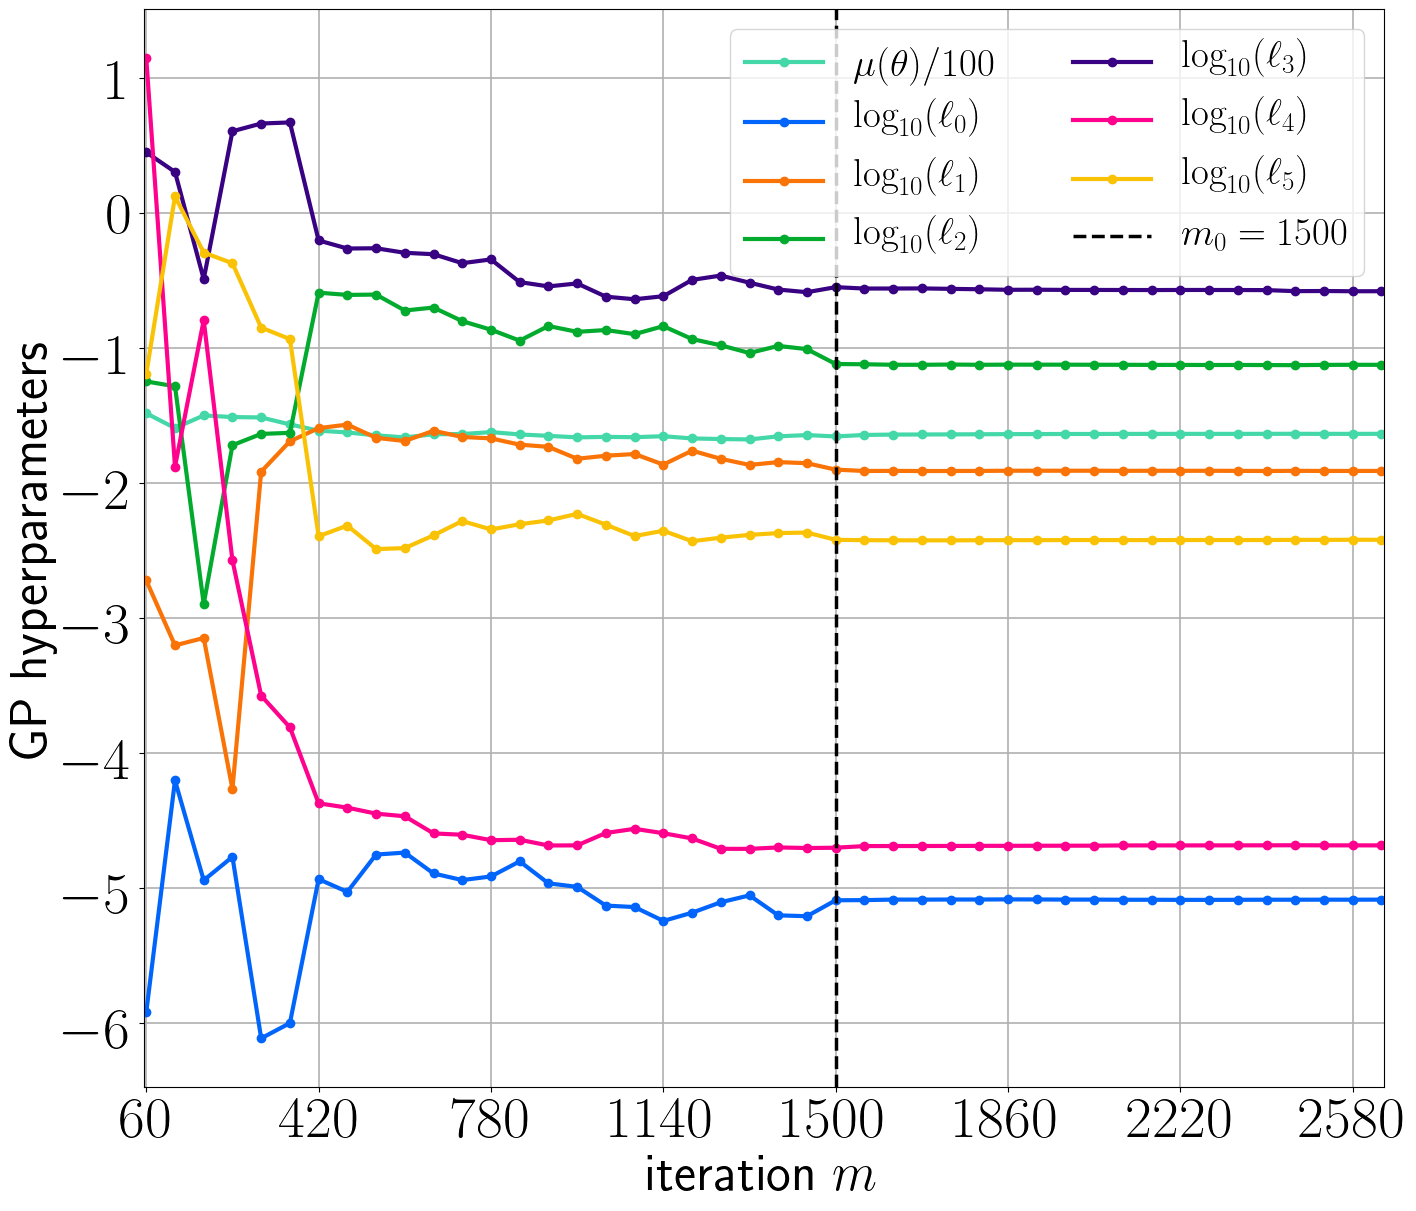
\includegraphics[width=0.47\textwidth]{figs/appendix/220808_014638_GP_hparams.png}
    \figcaption{\textbf{Hyperparameters of the GP over the course of training.} Hyperparameters include the mean value and covariance kernel length scales of the GP, $\ell_j$, in each dimension $j$ of $\theta$-space. The mean value is normalized by $10^2$ for legibility. The hyperparameters rapidly converge and then remain stable during construction of the base training set, indicating that the optimal hyperparameters have been found. Once active learning begins at $m = 1500$, the hyperparameters remain stable.}\label{fig:hparams}
\end{figure}


%%% === APPENDIX C === %%%
%% ABUNDANCES %%
\section{Detailed Ion Abundances}\label{app:ion_abunds}

In Tables~\ref{tab:ion_abunds_bluehot} and \ref{tab:ion_abunds_purplewarm}, we provide mass fractions and uncertainties for all of the relevant ions in the ejecta in our best-fit blue+hot and purple+warm models. The majority of elements are singly ionized. We also provide the total mass of each ion contained in our simulation, and, the mass of each ion under the assumption of some fiducial total ejecta mass of $0.02~M_{\odot}$ and uniform composition above and below the photosphere.






\startlongtable
\begin{deluxetable}{cc|c}
\tablewidth{\textwidth}
\centering
\tablecaption{Number of lines for each ion, for elements with $Z \geqslant 31$. For elements with $Z<31$, an additional 1,476,338 lines (dominated by the iron group) are used.}\label{tab:linecounts} 
\tablehead{\colhead{$Z$} & \colhead{ion} & \colhead{$N_{\mathrm{lines}}$}} 
\startdata
1-30 & H - Zn \ion{}{1}~-\ion{}{3}\tablenotemark{a} & 1,476,338 \\\hline
31 & \ion{Ga}{1} & 41 \\
 & \ion{Ga}{2} & 194 \\
 & \ion{Ga}{3} & 2 \\\hline
32 & \ion{Ge}{1} & 64 \\
 & \ion{Ge}{2} & 22 \\\hline
33 & \ion{As}{1} & 110 \\\hline
34 & \ion{Se}{1} & 8 \\\hline
37 & \ion{Rb}{1} & 143 \\\hline
38 & \ion{Sr}{1} & 110 \\
 & \ion{Sr}{2} & 695 \\\hline
39 & \ion{Y}{1} & 5,365 \\
 & \ion{Y}{2} & 7,753 \\
 & \ion{Y}{3} & 39 \\\hline
40 & \ion{Zr}{1} & 699 \\
 & \ion{Zr}{2} & 542 \\
 & \ion{Zr}{3} & 359 \\\hline
41 & \ion{Nb}{1} & 1,044 \\
 & \ion{Nb}{2} & 2,988 \\
 & \ion{Nb}{3} & 76 \\\hline
42 & \ion{Mo}{1} & 2,892 \\
 & \ion{Mo}{2} & 328 \\\hline
43 & \ion{Tc}{1} & 52 \\\hline
44 & \ion{Ru}{1} & 1,028 \\
 & \ion{Ru}{2} & 127  \\\hline
45 & \ion{Rh}{1} & 440 \\
 & \ion{Rh}{2} & 94 \\\hline
46 & \ion{Pd}{1} & 76 \\
 & \ion{Pd}{2} & 13 \\\hline
47 & \ion{Ag}{1} & 15 \\
 & \ion{Ag}{2} & 10 \\\hline
48 & \ion{Cd}{1} & 20  \\
 & \ion{Cd}{2} & 4 \\\hline
49 & \ion{In}{1} & 24 \\
 & \ion{In}{2} & 16 \\\hline
50 & \ion{Sn}{1} & 59 \\
 & \ion{Sn}{2} & 22 \\\hline
51 & \ion{Sb}{1} & 73 \\\hline
52 & \ion{Te}{1} & 18 \\\hline
54 & \ion{Xe}{2} & 33 \\\hline
55 & \ion{Cs}{1} & 150 \\\hline
56 & \ion{Ba}{1} & 125 \\
 & \ion{Ba}{2} & 244 \\\hline
57 & \ion{La}{1} & 267 \\
 & \ion{La}{2} & 3,938 \\
 & \ion{La}{3} & 131 \\\hline
58 & \ion{Ce}{1} & 903 \\
 & \ion{Ce}{2} & 16,014 \\
 & \ion{Ce}{3} & 3,023 \\\hline
59 & \ion{Pr}{1} & 127 \\
 & \ion{Pr}{2} & 7,723 \\
 & \ion{Pr}{3} & 1,151 \\\hline
60 & \ion{Nd}{1} & 281 \\
 & \ion{Nd}{2} & 1,279 \\
 & \ion{Nd}{3} & 71 \\\hline
62 & \ion{Sm}{1} & 520 \\
 & \ion{Sm}{2} & 1,334 \\
 & \ion{Sm}{3} & 49 \\\hline
63 & \ion{Eu}{1} & 352 \\
 & \ion{Eu}{2} & 871 \\
 & \ion{Eu}{3} & 1,150 \\\hline
64 & \ion{Gd}{1} & 620 \\
 & \ion{Gd}{2} & 963 \\
 & \ion{Gd}{3} & 52 \\\hline
65 & \ion{Tb}{1} & 3 \\
 & \ion{Tb}{2} & 1,822 \\
 & \ion{Tb}{3} & 80 \\\hline
66 & \ion{Dy}{1} & 834 \\
 & \ion{Dy}{2} & 897 \\
 & \ion{Dy}{3} & 1,337 \\\hline
67 & \ion{Ho}{1} & 711 \\
 & \ion{Ho}{2} & 496 \\
 & \ion{Ho}{3} & 1,309 \\\hline
68 & \ion{Er}{1} & 365 \\
 & \ion{Er}{2} & 775 \\
 & \ion{Er}{3} & 1,308 \\\hline
69 & \ion{Tm}{1} & 532 \\
 & \ion{Tm}{2} & 7,919 \\
 & \ion{Tm}{3} & 1,479 \\\hline
70 & \ion{Yb}{1} & 83 \\
 & \ion{Yb}{2} & 6,794  \\
 & \ion{Yb}{3} & 271 \\\hline
71 & \ion{Lu}{1} & 247 \\
 & \ion{Lu}{2} & 125 \\
 & \ion{Lu}{3} & 59 \\\hline
72 & \ion{Hf}{1} & 430 \\
 & \ion{Hf}{2} & 434 \\\hline
73 & \ion{Ta}{1} & 11,470 \\
 & \ion{Ta}{2} & 3,992 \\\hline
74 & \ion{W}{1} & 1,062 \\
 & \ion{W}{2} & 221 \\\hline
75 & \ion{Re}{1} & 772 \\
 & \ion{Re}{2} & 47 \\\hline
76 & \ion{Os}{1} & 891 \\
 & \ion{Os}{2} & 47 \\\hline
77 & \ion{Ir}{1} & 501 \\
 & \ion{Ir}{2} & 28 \\\hline
78 & \ion{Pt}{1} & 215 \\
 & \ion{Pt}{2} & 119 \\
 & \ion{Pt}{3} & 666 \\\hline
79 & \ion{Au}{1} & 61 \\
 & \ion{Au}{2} & 498 \\
 & \ion{Au}{3} & 175 \\\hline
80 & \ion{Hg}{1} & 27 \\
 & \ion{Hg}{2} & 446 \\
 & \ion{Hg}{3} & 42 \\\hline
81 & \ion{Tl}{1} & 22 \\\hline
82 & \ion{Pb}{1} & 38 \\
 & \ion{Pb}{2} & 60 \\\hline
83 & \ion{Bi}{1} & 29 \\
 & \ion{Bi}{2} & 14 \\\hline
90 & \ion{Th}{1} & 700 \\
 & \ion{Th}{2} & 1,448 \\
 & \ion{Th}{3} & 903 \\\hline
92 & \ion{U}{1} & 561 \\
 & \ion{U}{2} & 622 \\\hline
 & \textbf{TOTAL} & \textbf{1,597,376}  \\
\enddata
\tablenotetext{a}{Lines acquired as available: for some doubly-ionized iron-group elements, lines are not available.}
\end{deluxetable}




\startlongtable
\begin{deluxetable*}{cc|c|c|c}
\tablewidth{\textwidth}
\centering
\tablecaption{Mass fractions and masses for all ions in the blue+hot model with a mass fraction $\mathrm{X}_i \geqslant 10^{-9}$. Columns include the atomic number $Z$, the name of the ion, the mass fraction $\mathrm{X}_i$ of the ion, and the mass of the ion in our simulation, using our inferred lower bound on the ejecta mass $M_{\mathrm{ej}} > 3.5^{+4.2}_{-3.3} \times 10^{-5}~M_{\odot}$. We also include the mass of the ion assuming some fiducial total ejecta mass of $M_{\mathrm{ej}} = 0.02~M_{\odot}$ and a uniform composition above and below the photosphere. We highlight ions of interest: \ion{Sr}{2}, \ion{Y}{2}, and \ion{Zr}{2}. }\label{tab:ion_abunds_bluehot} 
\tablehead{\colhead{$Z$} & \colhead{ion} & \colhead{mass fraction $\mathrm{X}_i$} & \colhead{lower bound $M_{\mathrm{ej,i}}~[M_{\odot}]$} & \colhead{fiducial $M_{0.02,\mathrm{i}}$} } 
\startdata
1 & \ion{H}{1} & ${5.01}^{+0.04}_{-1.00} \times 10^{-5}$ & ${1.75}^{+1.20}_{-1.37} \times 10^{-9}$ & ${1.00}^{+0.04}_{-1.00} \times 10^{-6}$ \\
 & \ion{H}{2} & ${4.75}^{+0.04}_{-1.00} \times 10^{-7}$ & ${1.66}^{+1.20}_{-1.37} \times 10^{-11}$ & ${9.51}^{+0.04}_{-1.00} \times 10^{-9}$ \\\hline
2 & \ion{He}{1} & ${8.36}^{+4.03}_{-1.00} \times 10^{-1}$ & ${2.93}^{+4.21}_{-1.37} \times 10^{-5}$ & ${1.67}^{+4.03}_{-1.00} \times 10^{-2}$ \\\hline
3 & \ion{Li}{2} & ${2.49}^{+0.55}_{-1.00} \times 10^{-8}$ & ${8.72}^{+1.32}_{-1.37} \times 10^{-13}$ & ${4.98}^{+0.55}_{-1.00} \times 10^{-10}$ \\\hline
4 & \ion{Be}{2} & ${8.53}^{+0.55}_{-1.00} \times 10^{-9}$ & ${2.98}^{+1.32}_{-1.37} \times 10^{-13}$ & ${1.71}^{+0.55}_{-1.00} \times 10^{-10}$ \\\hline
6 & \ion{C}{1} & ${3.49}^{+356.60}_{-1.00} \times 10^{-7}$ & ${1.22}^{+356.60}_{-1.37} \times 10^{-11}$ & ${6.97}^{+356.60}_{-1.00} \times 10^{-9}$ \\
 & \ion{C}{2} & ${4.63}^{+356.60}_{-1.00} \times 10^{-6}$ & ${1.62}^{+356.60}_{-1.37} \times 10^{-10}$ & ${9.26}^{+356.60}_{-1.00} \times 10^{-8}$ \\\hline
7 & \ion{N}{1} & ${5.16}^{+356.60}_{-1.00} \times 10^{-8}$ & ${1.81}^{+356.60}_{-1.37} \times 10^{-12}$ & ${1.03}^{+356.60}_{-1.00} \times 10^{-9}$ \\\hline
8 & \ion{O}{1} & ${7.72}^{+12.24}_{-1.00} \times 10^{-7}$ & ${2.70}^{+12.30}_{-1.37} \times 10^{-11}$ & ${1.54}^{+12.24}_{-1.00} \times 10^{-8}$ \\
 & \ion{O}{2} & ${6.30}^{+12.24}_{-1.00} \times 10^{-9}$ & ${2.20}^{+12.30}_{-1.37} \times 10^{-13}$ & ${1.26}^{+12.24}_{-1.00} \times 10^{-10}$ \\\hline
9 & \ion{F}{1} & ${9.59}^{+14.04}_{-1.00} \times 10^{-6}$ & ${3.36}^{+14.09}_{-1.37} \times 10^{-10}$ & ${1.92}^{+14.04}_{-1.00} \times 10^{-7}$ \\\hline
10 & \ion{Ne}{1} & ${2.94}^{+14.04}_{-1.00} \times 10^{-7}$ & ${1.03}^{+14.09}_{-1.37} \times 10^{-11}$ & ${5.88}^{+14.04}_{-1.00} \times 10^{-9}$ \\\hline
11 & \ion{Na}{2} & ${1.93}^{+33.94}_{-1.00} \times 10^{-7}$ & ${6.76}^{+33.96}_{-1.37} \times 10^{-12}$ & ${3.86}^{+33.94}_{-1.00} \times 10^{-9}$ \\\hline
12 & \ion{Mg}{2} & ${5.89}^{+33.94}_{-1.00} \times 10^{-7}$ & ${2.06}^{+33.96}_{-1.37} \times 10^{-11}$ & ${1.18}^{+33.94}_{-1.00} \times 10^{-8}$ \\\hline
13 & \ion{Al}{2} & ${6.60}^{+12.79}_{-1.00} \times 10^{-8}$ & ${2.31}^{+12.85}_{-1.37} \times 10^{-12}$ & ${1.32}^{+12.79}_{-1.00} \times 10^{-9}$ \\\hline
14 & \ion{Si}{2} & ${5.21}^{+12.79}_{-1.00} \times 10^{-7}$ & ${1.82}^{+12.85}_{-1.37} \times 10^{-11}$ & ${1.04}^{+12.79}_{-1.00} \times 10^{-8}$ \\\hline
15 & \ion{P}{1} & ${1.34}^{+12.69}_{-1.00} \times 10^{-9}$ & ${4.68}^{+12.74}_{-1.37} \times 10^{-14}$ & ${2.68}^{+12.69}_{-1.00} \times 10^{-11}$ \\
 & \ion{P}{2} & ${5.39}^{+6.06}_{-1.00} \times 10^{-7}$ & ${1.89}^{+6.18}_{-1.37} \times 10^{-11}$ & ${1.08}^{+6.06}_{-1.00} \times 10^{-8}$ \\\hline
16 & \ion{S}{1} & ${1.07}^{+6.06}_{-1.00} \times 10^{-8}$ & ${3.74}^{+6.18}_{-1.37} \times 10^{-13}$ & ${2.14}^{+6.06}_{-1.00} \times 10^{-10}$ \\
 & \ion{S}{2} & ${1.34}^{+3.52}_{-1.00} \times 10^{-6}$ & ${4.70}^{+3.72}_{-1.37} \times 10^{-11}$ & ${2.68}^{+3.52}_{-1.00} \times 10^{-8}$ \\\hline
17 & \ion{Cl}{1} & ${4.09}^{+3.52}_{-1.00} \times 10^{-8}$ & ${1.43}^{+3.72}_{-1.37} \times 10^{-12}$ & ${8.17}^{+3.52}_{-1.00} \times 10^{-10}$ \\
 & \ion{Cl}{2} & ${7.55}^{+3.52}_{-1.00} \times 10^{-9}$ & ${2.64}^{+3.72}_{-1.37} \times 10^{-13}$ & ${1.51}^{+3.52}_{-1.00} \times 10^{-10}$ \\\hline
18 & \ion{Ar}{1} & ${2.05}^{+1.41}_{-1.00} \times 10^{-7}$ & ${7.16}^{+1.85}_{-1.37} \times 10^{-12}$ & ${4.09}^{+1.41}_{-1.00} \times 10^{-9}$ \\\hline
19 & \ion{K}{2} & ${1.48}^{+1.41}_{-1.00} \times 10^{-7}$ & ${5.17}^{+1.85}_{-1.37} \times 10^{-12}$ & ${2.96}^{+1.41}_{-1.00} \times 10^{-9}$ \\\hline
20 & \ion{Ca}{2} & ${7.18}^{+1.41}_{-1.00} \times 10^{-8}$ & ${2.51}^{+1.85}_{-1.37} \times 10^{-12}$ & ${1.44}^{+1.41}_{-1.00} \times 10^{-9}$ \\
 & \ion{Ca}{3} & ${1.10}^{+5.15}_{-1.00} \times 10^{-7}$ & ${3.86}^{+5.29}_{-1.37} \times 10^{-12}$ & ${2.21}^{+5.15}_{-1.00} \times 10^{-9}$ \\\hline
21 & \ion{Sc}{2} & ${6.07}^{+5.15}_{-1.00} \times 10^{-9}$ & ${2.13}^{+5.29}_{-1.37} \times 10^{-13}$ & ${1.21}^{+5.15}_{-1.00} \times 10^{-10}$ \\\hline
22 & \ion{Ti}{2} & ${3.45}^{+5.15}_{-1.00} \times 10^{-8}$ & ${1.21}^{+5.29}_{-1.37} \times 10^{-12}$ & ${6.89}^{+5.15}_{-1.00} \times 10^{-10}$ \\\hline
23 & \ion{V}{2} & ${1.88}^{+17.02}_{-1.00} \times 10^{-7}$ & ${6.59}^{+17.06}_{-1.37} \times 10^{-12}$ & ${3.76}^{+17.02}_{-1.00} \times 10^{-9}$ \\\hline
24 & \ion{Cr}{2} & ${9.65}^{+17.02}_{-1.00} \times 10^{-5}$ & ${3.38}^{+17.06}_{-1.37} \times 10^{-9}$ & ${1.93}^{+17.02}_{-1.00} \times 10^{-6}$ \\
 & \ion{Cr}{3} & ${1.16}^{+20.41}_{-1.00} \times 10^{-9}$ & ${4.04}^{+20.45}_{-1.37} \times 10^{-14}$ & ${2.31}^{+20.41}_{-1.00} \times 10^{-11}$ \\\hline
25 & \ion{Mn}{2} & ${6.20}^{+20.41}_{-1.00} \times 10^{-6}$ & ${2.17}^{+20.45}_{-1.37} \times 10^{-10}$ & ${1.24}^{+20.41}_{-1.00} \times 10^{-7}$ \\\hline
26 & \ion{Fe}{2} & ${3.66}^{+46.99}_{-1.00} \times 10^{-5}$ & ${1.28}^{+47.01}_{-1.37} \times 10^{-9}$ & ${7.32}^{+46.99}_{-1.00} \times 10^{-7}$ \\\hline
27 & \ion{Co}{2} & ${1.24}^{+46.99}_{-1.00} \times 10^{-7}$ & ${4.35}^{+47.01}_{-1.37} \times 10^{-12}$ & ${2.48}^{+46.99}_{-1.00} \times 10^{-9}$ \\\hline
28 & \ion{Ni}{2} & ${1.00}^{+34.30}_{-1.00} \times 10^{-4}$ & ${3.51}^{+34.32}_{-1.37} \times 10^{-9}$ & ${2.00}^{+34.30}_{-1.00} \times 10^{-6}$ \\\hline
29 & \ion{Cu}{2} & ${2.54}^{+34.30}_{-1.00} \times 10^{-5}$ & ${8.90}^{+34.32}_{-1.37} \times 10^{-10}$ & ${5.09}^{+34.30}_{-1.00} \times 10^{-7}$ \\\hline
30 & \ion{Zn}{1} & ${7.42}^{+73.25}_{-1.00} \times 10^{-9}$ & ${2.60}^{+73.26}_{-1.37} \times 10^{-13}$ & ${1.48}^{+73.25}_{-1.00} \times 10^{-10}$ \\
 & \ion{Zn}{2} & ${7.86}^{+3698.81}_{-0.86} \times 10^{-5}$ & ${2.75}^{+3698.81}_{-1.28} \times 10^{-9}$ & ${1.57}^{+3698.81}_{-0.86} \times 10^{-6}$ \\\hline
31 & \ion{Ga}{2} & ${2.27}^{+3698.81}_{-0.86} \times 10^{-5}$ & ${7.93}^{+3698.81}_{-1.28} \times 10^{-10}$ & ${4.53}^{+3698.81}_{-0.86} \times 10^{-7}$ \\\hline
32 & \ion{Ge}{2} & ${1.30}^{+3698.81}_{-0.86} \times 10^{-4}$ & ${4.54}^{+3698.81}_{-1.28} \times 10^{-9}$ & ${2.59}^{+3698.81}_{-0.86} \times 10^{-6}$ \\\hline
33 & \ion{As}{1} & ${2.95}^{+1118.47}_{-1.00} \times 10^{-7}$ & ${1.03}^{+1118.47}_{-1.37} \times 10^{-11}$ & ${5.91}^{+1118.47}_{-1.00} \times 10^{-9}$ \\
 & \ion{As}{2} & ${1.15}^{+1118.47}_{-1.00} \times 10^{-4}$ & ${4.03}^{+1118.47}_{-1.37} \times 10^{-9}$ & ${2.30}^{+1118.47}_{-1.00} \times 10^{-6}$ \\\hline
34 & \ion{Se}{1} & ${1.01}^{+1118.47}_{-1.00} \times 10^{-5}$ & ${3.53}^{+1118.47}_{-1.37} \times 10^{-10}$ & ${2.02}^{+1118.47}_{-1.00} \times 10^{-7}$ \\
& \ion{Se}{2} & ${1.07}^{+18627.73}_{-0.98} \times 10^{-2}$ & ${3.76}^{+18627.73}_{-1.36} \times 10^{-7}$ & ${2.15}^{+18627.73}_{-0.98} \times 10^{-4}$ \\\hline
35 & \ion{Br}{1} & ${2.14}^{+18627.73}_{-0.98} \times 10^{-4}$ & ${7.48}^{+18627.73}_{-1.36} \times 10^{-9}$ & ${4.28}^{+18627.73}_{-0.98} \times 10^{-6}$ \\
& \ion{Br}{2} & ${1.04}^{+18627.73}_{-0.98} \times 10^{-3}$ & ${3.64}^{+18627.73}_{-1.36} \times 10^{-8}$ & ${2.08}^{+18627.73}_{-0.98} \times 10^{-5}$ \\\hline
36 & \ion{Kr}{1} & ${4.06}^{+5859.54}_{-0.99} \times 10^{-2}$ & ${1.42}^{+5859.54}_{-1.37} \times 10^{-6}$ & ${8.12}^{+5859.54}_{-0.99} \times 10^{-4}$ \\
& \ion{Kr}{2} & ${9.31}^{+5859.54}_{-0.99} \times 10^{-4}$ & ${3.26}^{+5859.54}_{-1.37} \times 10^{-8}$ & ${1.86}^{+5859.54}_{-0.99} \times 10^{-5}$ \\\hline
37 & \ion{Rb}{2} & ${2.53}^{+5859.54}_{-0.99} \times 10^{-2}$ & ${8.84}^{+5859.54}_{-1.37} \times 10^{-7}$ & ${5.05}^{+5859.54}_{-0.99} \times 10^{-4}$ \\\hline
38 & \textbf{\ion{Sr}{2}} & $\mathbf{{1.35}^{+920.70}_{-1.00} \times 10^{-3}}$ & $\mathbf{{4.72}^{+920.70}_{-1.37} \times 10^{-8}}$ & $\mathbf{{2.70}^{+920.70}_{-1.00} \times 10^{-5}}$ \\
& \ion{Sr}{3} & ${2.65}^{+920.70}_{-1.00} \times 10^{-2}$ & ${9.29}^{+920.70}_{-1.37} \times 10^{-7}$ & ${5.31}^{+920.70}_{-1.00} \times 10^{-4}$ \\\hline
39 & \textbf{\ion{Y}{2}} & $\mathbf{{3.55}^{+920.70}_{-1.00} \times 10^{-3}}$ & $\mathbf{{1.24}^{+920.70}_{-1.37} \times 10^{-7}}$ & $\mathbf{{7.10}^{+920.70}_{-1.00} \times 10^{-5}}$ \\
& \ion{Y}{3} & ${2.68}^{+298.76}_{-1.00} \times 10^{-3}$ & ${9.37}^{+298.76}_{-1.37} \times 10^{-8}$ & ${5.35}^{+298.76}_{-1.00} \times 10^{-5}$ \\\hline
40 & \ion{Zr}{1} & ${1.23}^{+298.76}_{-1.00} \times 10^{-9}$ & ${4.31}^{+298.76}_{-1.37} \times 10^{-14}$ & ${2.46}^{+298.76}_{-1.00} \times 10^{-11}$ \\
& \textbf{\ion{Zr}{2}} & $\mathbf{ {3.50}^{+298.76}_{-1.00} \times 10^{-2} }$ & $\mathbf{{1.23}^{+298.76}_{-1.37} \times 10^{-6}}$ & $\mathbf{ {7.01}^{+298.76}_{-1.00} \times 10^{-4} }$ \\
& \ion{Zr}{3} & ${1.24}^{+318.33}_{-1.00} \times 10^{-3}$ & ${4.33}^{+318.34}_{-1.37} \times 10^{-8}$ & ${2.48}^{+318.33}_{-1.00} \times 10^{-5}$ \\\hline
41 & \ion{Nb}{2} & ${7.49}^{+318.33}_{-1.00} \times 10^{-5}$ & ${2.62}^{+318.34}_{-1.37} \times 10^{-9}$ & ${1.50}^{+318.33}_{-1.00} \times 10^{-6}$ \\
& \ion{Nb}{3} & ${5.13}^{+318.33}_{-1.00} \times 10^{-8}$ & ${1.80}^{+318.34}_{-1.37} \times 10^{-12}$ & ${1.03}^{+318.33}_{-1.00} \times 10^{-9}$ \\\hline
42 & \ion{Mo}{2} & ${4.40}^{+456.69}_{-1.00} \times 10^{-3}$ & ${1.54}^{+456.69}_{-1.37} \times 10^{-7}$ & ${8.80}^{+456.69}_{-1.00} \times 10^{-5}$ \\
& \ion{Mo}{3} & ${5.93}^{+456.69}_{-1.00} \times 10^{-9}$ & ${2.08}^{+456.69}_{-1.37} \times 10^{-13}$ & ${1.19}^{+456.69}_{-1.00} \times 10^{-10}$ \\\hline
43 & \ion{Tc}{2} & ${2.18}^{+456.69}_{-1.00} \times 10^{-4}$ & ${7.64}^{+456.69}_{-1.37} \times 10^{-9}$ & ${4.37}^{+456.69}_{-1.00} \times 10^{-6}$ \\
& \ion{Tc}{3} & ${2.50}^{+203.20}_{-1.00} \times 10^{-8}$ & ${8.74}^{+203.20}_{-1.37} \times 10^{-13}$ & ${4.99}^{+203.20}_{-1.00} \times 10^{-10}$ \\\hline
44 & \ion{Ru}{1} & ${5.54}^{+203.20}_{-1.00} \times 10^{-9}$ & ${1.94}^{+203.20}_{-1.37} \times 10^{-13}$ & ${1.11}^{+203.20}_{-1.00} \times 10^{-10}$ \\
& \ion{Ru}{2} & ${7.20}^{+203.20}_{-1.00} \times 10^{-3}$ & ${2.52}^{+203.20}_{-1.37} \times 10^{-7}$ & ${1.44}^{+203.20}_{-1.00} \times 10^{-4}$ \\
& \ion{Ru}{3} & ${5.07}^{+179.83}_{-1.00} \times 10^{-9}$ & ${1.77}^{+179.83}_{-1.37} \times 10^{-13}$ & ${1.01}^{+179.83}_{-1.00} \times 10^{-10}$ \\\hline
45 & \ion{Rh}{2} & ${5.23}^{+179.83}_{-1.00} \times 10^{-4}$ & ${1.83}^{+179.83}_{-1.37} \times 10^{-8}$ & ${1.05}^{+179.83}_{-1.00} \times 10^{-5}$ \\\hline
46 & \ion{Pd}{1} & ${2.55}^{+115.22}_{-1.00} \times 10^{-9}$ & ${8.91}^{+115.23}_{-1.37} \times 10^{-14}$ & ${5.09}^{+115.22}_{-1.00} \times 10^{-11}$ \\
& \ion{Pd}{2} & ${1.10}^{+115.22}_{-1.00} \times 10^{-3}$ & ${3.84}^{+115.23}_{-1.37} \times 10^{-8}$ & ${2.19}^{+115.22}_{-1.00} \times 10^{-5}$ \\\hline
47 & \ion{Ag}{2} & ${2.55}^{+115.22}_{-1.00} \times 10^{-4}$ & ${8.94}^{+115.23}_{-1.37} \times 10^{-9}$ & ${5.11}^{+115.22}_{-1.00} \times 10^{-6}$ \\\hline
48 & \ion{Cd}{1} & ${6.49}^{+94.70}_{-1.00} \times 10^{-9}$ & ${2.27}^{+94.71}_{-1.37} \times 10^{-13}$ & ${1.30}^{+94.70}_{-1.00} \times 10^{-10}$ \\
& \ion{Cd}{2} & ${2.27}^{+94.70}_{-1.00} \times 10^{-4}$ & ${7.95}^{+94.71}_{-1.37} \times 10^{-9}$ & ${4.54}^{+94.70}_{-1.00} \times 10^{-6}$ \\\hline
49 & \ion{In}{2} & ${6.99}^{+208.53}_{-1.00} \times 10^{-6}$ & ${2.45}^{+208.54}_{-1.37} \times 10^{-10}$ & ${1.40}^{+208.53}_{-1.00} \times 10^{-7}$ \\\hline
50 & \ion{Sn}{2} & ${6.25}^{+208.53}_{-1.00} \times 10^{-5}$ & ${2.19}^{+208.54}_{-1.37} \times 10^{-9}$ & ${1.25}^{+208.53}_{-1.00} \times 10^{-6}$ \\
& \ion{Sn}{3} & ${1.91}^{+208.53}_{-1.00} \times 10^{-8}$ & ${6.70}^{+208.54}_{-1.37} \times 10^{-13}$ & ${3.83}^{+208.53}_{-1.00} \times 10^{-10}$ \\\hline
51 & \ion{Sb}{2} & ${9.76}^{+38.01}_{-1.00} \times 10^{-6}$ & ${3.42}^{+38.03}_{-1.37} \times 10^{-10}$ & ${1.95}^{+38.01}_{-1.00} \times 10^{-7}$ \\\hline
52 & \ion{Te}{2} & ${7.71}^{+38.01}_{-1.00} \times 10^{-6}$ & ${2.70}^{+38.03}_{-1.37} \times 10^{-10}$ & ${1.54}^{+38.01}_{-1.00} \times 10^{-7}$ \\\hline
53 & \ion{I}{1} & ${1.07}^{+38.01}_{-1.00} \times 10^{-8}$ & ${3.74}^{+38.03}_{-1.37} \times 10^{-13}$ & ${2.14}^{+38.01}_{-1.00} \times 10^{-10}$ \\
& \ion{I}{2} & ${3.03}^{+9.27}_{-1.00} \times 10^{-6}$ & ${1.06}^{+9.35}_{-1.37} \times 10^{-10}$ & ${6.05}^{+9.27}_{-1.00} \times 10^{-8}$ \\\hline
54 & \ion{Xe}{1} & ${1.27}^{+9.27}_{-1.00} \times 10^{-9}$ & ${4.43}^{+9.35}_{-1.37} \times 10^{-14}$ & ${2.53}^{+9.27}_{-1.00} \times 10^{-11}$ \\
& \ion{Xe}{2} & ${7.68}^{+24.70}_{-1.00} \times 10^{-9}$ & ${2.69}^{+24.73}_{-1.37} \times 10^{-13}$ & ${1.54}^{+24.70}_{-1.00} \times 10^{-10}$
\enddata
\end{deluxetable*}


\startlongtable
\begin{deluxetable*}{cc|c|c|c}
\tablewidth{\textwidth}
\centering
\tablecaption{Same as Table~\ref{tab:ion_abunds_bluehot}, for the purple+warm best-fitting model. The lower bound on the total ejecta mass, which is used to compute the mass of each ion in the simulation, is $M_{\mathrm{ej}} > 4.0^{+2.9}_{-2.9} \times 10^{-5}~M_{\odot}$ for this model. We highlight ions of interest: \ion{Sr}{2}, \ion{Y}{2}, and \ion{Zr}{2}. }\label{tab:ion_abunds_purplewarm} 
\tablehead{\colhead{$Z$} & \colhead{ion} & \colhead{mass fraction $\mathrm{X}_i$} & \colhead{lower bound $M_{\mathrm{ej,i}}~[M_{\odot}]$} & \colhead{fiducial $M_{0.02,\mathrm{i}}$} } 
\startdata
1 & \ion{H}{1} & ${1.69}^{+1.93}_{-0.78} \times 10^{-4}$ & ${6.74}^{+2.06}_{-1.07} \times 10^{-9}$ & ${3.37}^{+1.93}_{-0.78} \times 10^{-6}$ \\
& \ion{H}{2} & ${8.27}^{+1.93}_{-0.78} \times 10^{-7}$ & ${3.31}^{+2.06}_{-1.07} \times 10^{-11}$ & ${1.65}^{+1.93}_{-0.78} \times 10^{-8}$ \\\hline
2 & \ion{He}{1} & ${6.79}^{+1.20}_{-0.50} \times 10^{-2}$ & ${2.72}^{+1.40}_{-0.88} \times 10^{-6}$ & ${1.36}^{+1.20}_{-0.50} \times 10^{-3}$ \\\hline
3 & \ion{Li}{2} & ${1.34}^{+0.90}_{-0.50} \times 10^{-7}$ & ${5.34}^{+1.16}_{-0.88} \times 10^{-12}$ & ${2.67}^{+0.90}_{-0.50} \times 10^{-9}$ \\\hline
4 & \ion{Be}{1} & ${8.10}^{+0.90}_{-0.50} \times 10^{-9}$ & ${3.24}^{+1.16}_{-0.88} \times 10^{-13}$ & ${1.62}^{+0.90}_{-0.50} \times 10^{-10}$ \\
& \ion{Be}{2} & ${5.56}^{+1.22}_{-0.58} \times 10^{-5}$ & ${2.23}^{+1.42}_{-0.93} \times 10^{-9}$ & ${1.11}^{+1.22}_{-0.58} \times 10^{-6}$ \\\hline
5 & \ion{B}{2} & ${5.45}^{+1.22}_{-0.58} \times 10^{-8}$ & ${2.18}^{+1.42}_{-0.93} \times 10^{-12}$ & ${1.09}^{+1.22}_{-0.58} \times 10^{-9}$ \\\hline
6 & \ion{C}{1} & ${3.06}^{+1.22}_{-0.58} \times 10^{-7}$ & ${1.22}^{+1.42}_{-0.93} \times 10^{-11}$ & ${6.11}^{+1.22}_{-0.58} \times 10^{-9}$ \\
& \ion{C}{2} & ${2.12}^{+1.39}_{-0.66} \times 10^{-6}$ & ${8.47}^{+1.57}_{-0.98} \times 10^{-11}$ & ${4.23}^{+1.39}_{-0.66} \times 10^{-8}$ \\\hline
7 & \ion{N}{1} & ${2.01}^{+1.39}_{-0.66} \times 10^{-8}$ & ${8.02}^{+1.57}_{-0.98} \times 10^{-13}$ & ${4.01}^{+1.39}_{-0.66} \times 10^{-10}$ \\\hline
8 & \ion{O}{1} & ${1.11}^{+4.42}_{-0.74} \times 10^{-6}$ & ${4.45}^{+4.48}_{-1.03} \times 10^{-11}$ & ${2.23}^{+4.42}_{-0.74} \times 10^{-8}$ \\
& \ion{O}{2} & ${4.70}^{+4.42}_{-0.74} \times 10^{-9}$ & ${1.88}^{+4.48}_{-1.03} \times 10^{-13}$ & ${9.40}^{+4.42}_{-0.74} \times 10^{-11}$ \\\hline
9 & \ion{F}{1} & ${1.20}^{+18.89}_{-0.89} \times 10^{-8}$ & ${4.78}^{+18.91}_{-1.15} \times 10^{-13}$ & ${2.39}^{+18.89}_{-0.89} \times 10^{-10}$ \\\hline
20 & \ion{Ca}{2} & ${6.75}^{+18.89}_{-0.89} \times 10^{-7}$ & ${2.70}^{+18.91}_{-1.15} \times 10^{-11}$ & ${1.35}^{+18.89}_{-0.89} \times 10^{-8}$ \\
& \ion{Ca}{3} & ${5.41}^{+6.35}_{-0.81} \times 10^{-7}$ & ${2.16}^{+6.39}_{-1.08} \times 10^{-11}$ & ${1.08}^{+6.35}_{-0.81} \times 10^{-8}$ \\\hline
21 & \ion{Sc}{2} & ${2.17}^{+6.35}_{-0.81} \times 10^{-8}$ & ${8.70}^{+6.39}_{-1.08} \times 10^{-13}$ & ${4.35}^{+6.35}_{-0.81} \times 10^{-10}$ \\\hline
22 & \ion{Ti}{2} & ${1.05}^{+17.53}_{-0.88} \times 10^{-5}$ & ${4.21}^{+17.54}_{-1.14} \times 10^{-10}$ & ${2.11}^{+17.53}_{-0.88} \times 10^{-7}$ \\
& \ion{Ti}{3} & ${4.27}^{+17.53}_{-0.88} \times 10^{-8}$ & ${1.71}^{+17.54}_{-1.14} \times 10^{-12}$ & ${8.53}^{+17.53}_{-0.88} \times 10^{-10}$ \\\hline
23 & \ion{V}{2} & ${1.28}^{+2.72}_{-0.92} \times 10^{-4}$ & ${5.14}^{+2.81}_{-1.17} \times 10^{-9}$ & ${2.57}^{+2.72}_{-0.92} \times 10^{-6}$ \\
& \ion{V}{3} & ${2.58}^{+2.72}_{-0.92} \times 10^{-8}$ & ${1.03}^{+2.81}_{-1.17} \times 10^{-12}$ & ${5.17}^{+2.72}_{-0.92} \times 10^{-10}$ \\\hline
24 & \ion{Cr}{1} & ${4.43}^{+2.72}_{-0.92} \times 10^{-8}$ & ${1.77}^{+2.81}_{-1.17} \times 10^{-12}$ & ${8.85}^{+2.72}_{-0.92} \times 10^{-10}$ \\
& \ion{Cr}{2} & ${2.33}^{+4.41}_{-0.94} \times 10^{-1}$ & ${9.31}^{+4.47}_{-1.19} \times 10^{-6}$ & ${4.65}^{+4.41}_{-0.94} \times 10^{-3}$ \\
& \ion{Cr}{3} & ${1.43}^{+4.41}_{-0.94} \times 10^{-6}$ & ${5.71}^{+4.47}_{-1.19} \times 10^{-11}$ & ${2.85}^{+4.41}_{-0.94} \times 10^{-8}$ \\\hline
25 & \ion{Mn}{1} & ${6.86}^{+4.41}_{-0.94} \times 10^{-9}$ & ${2.75}^{+4.47}_{-1.19} \times 10^{-13}$ & ${1.37}^{+4.41}_{-0.94} \times 10^{-10}$ \\
& \ion{Mn}{2} & ${7.89}^{+62.39}_{-0.99} \times 10^{-3}$ & ${3.16}^{+62.39}_{-1.23} \times 10^{-7}$ & ${1.58}^{+62.39}_{-0.99} \times 10^{-4}$ \\
& \ion{Mn}{3} & ${1.44}^{+62.39}_{-0.99} \times 10^{-7}$ & ${5.76}^{+62.39}_{-1.23} \times 10^{-12}$ & ${2.88}^{+62.39}_{-0.99} \times 10^{-9}$ \\\hline
26 & \ion{Fe}{1} & ${2.45}^{+62.39}_{-0.99} \times 10^{-7}$ & ${9.78}^{+62.39}_{-1.23} \times 10^{-12}$ & ${4.89}^{+62.39}_{-0.99} \times 10^{-9}$ \\
& \ion{Fe}{2} & ${9.32}^{+22.49}_{-0.76} \times 10^{-2}$ & ${3.73}^{+22.51}_{-1.05} \times 10^{-6}$ & ${1.86}^{+22.49}_{-0.76} \times 10^{-3}$ \\
& \ion{Fe}{3} & ${2.17}^{+22.49}_{-0.76} \times 10^{-7}$ & ${8.66}^{+22.51}_{-1.05} \times 10^{-12}$ & ${4.33}^{+22.49}_{-0.76} \times 10^{-9}$ \\\hline
27 & \ion{Co}{1} & ${1.12}^{+22.49}_{-0.76} \times 10^{-9}$ & ${4.48}^{+22.51}_{-1.05} \times 10^{-14}$ & ${2.24}^{+22.49}_{-0.76} \times 10^{-11}$ \\
& \ion{Co}{2} & ${1.77}^{+0.60}_{-0.56} \times 10^{-4}$ & ${7.07}^{+0.94}_{-0.92} \times 10^{-9}$ & ${3.54}^{+0.60}_{-0.56} \times 10^{-6}$ \\\hline
28 & \ion{Ni}{1} & ${7.32}^{+0.60}_{-0.56} \times 10^{-7}$ & ${2.93}^{+0.94}_{-0.92} \times 10^{-11}$ & ${1.46}^{+0.60}_{-0.56} \times 10^{-8}$ \\
& \ion{Ni}{2} & ${1.24}^{+0.60}_{-0.56} \times 10^{-1}$ & ${4.98}^{+0.94}_{-0.92} \times 10^{-6}$ & ${2.49}^{+0.60}_{-0.56} \times 10^{-3}$ \\
& \ion{Ni}{3} & ${2.40}^{+1.69}_{-0.58} \times 10^{-9}$ & ${9.59}^{+1.84}_{-0.93} \times 10^{-14}$ & ${4.79}^{+1.69}_{-0.58} \times 10^{-11}$ \\\hline
29 & \ion{Cu}{1} & ${8.23}^{+1.69}_{-0.58} \times 10^{-8}$ & ${3.29}^{+1.84}_{-0.93} \times 10^{-12}$ & ${1.65}^{+1.69}_{-0.58} \times 10^{-9}$ \\
& \ion{Cu}{2} & ${1.51}^{+1.69}_{-0.58} \times 10^{-2}$ & ${6.03}^{+1.84}_{-0.93} \times 10^{-7}$ & ${3.02}^{+1.69}_{-0.58} \times 10^{-4}$ \\\hline
30 & \ion{Zn}{1} & ${7.30}^{+0.53}_{-0.60} \times 10^{-6}$ & ${2.92}^{+0.90}_{-0.94} \times 10^{-10}$ & ${1.46}^{+0.53}_{-0.60} \times 10^{-7}$ \\
& \ion{Zn}{2} & ${4.06}^{+0.53}_{-0.60} \times 10^{-2}$ & ${1.62}^{+0.90}_{-0.94} \times 10^{-6}$ & ${8.12}^{+0.53}_{-0.60} \times 10^{-4}$ \\\hline
31 & \ion{Ga}{1} & ${1.16}^{+0.53}_{-0.60} \times 10^{-9}$ & ${4.62}^{+0.90}_{-0.94} \times 10^{-14}$ & ${2.31}^{+0.53}_{-0.60} \times 10^{-11}$ \\
& \ion{Ga}{2} & ${1.64}^{+0.43}_{-0.56} \times 10^{-2}$ & ${6.58}^{+0.84}_{-0.92} \times 10^{-7}$ & ${3.29}^{+0.43}_{-0.56} \times 10^{-4}$ \\\hline
32 & \ion{Ge}{1} & ${2.66}^{+0.43}_{-0.56} \times 10^{-7}$ & ${1.07}^{+0.84}_{-0.92} \times 10^{-11}$ & ${5.33}^{+0.43}_{-0.56} \times 10^{-9}$ \\
& \ion{Ge}{2} & ${3.88}^{+0.43}_{-0.56} \times 10^{-2}$ & ${1.55}^{+0.84}_{-0.92} \times 10^{-6}$ & ${7.76}^{+0.43}_{-0.56} \times 10^{-4}$ \\
& \ion{Ge}{3} & ${8.71}^{+0.67}_{-0.63} \times 10^{-8}$ & ${3.49}^{+0.98}_{-0.96} \times 10^{-12}$ & ${1.74}^{+0.67}_{-0.63} \times 10^{-9}$ \\\hline
33 & \ion{As}{1} & ${2.67}^{+0.67}_{-0.63} \times 10^{-5}$ & ${1.07}^{+0.98}_{-0.96} \times 10^{-9}$ & ${5.33}^{+0.67}_{-0.63} \times 10^{-7}$ \\
& \ion{As}{2} & ${5.45}^{+0.67}_{-0.63} \times 10^{-3}$ & ${2.18}^{+0.98}_{-0.96} \times 10^{-7}$ & ${1.09}^{+0.67}_{-0.63} \times 10^{-4}$ \\\hline
34 & \ion{Se}{1} & ${1.00}^{+0.80}_{-0.59} \times 10^{-4}$ & ${4.01}^{+1.08}_{-0.93} \times 10^{-9}$ & ${2.01}^{+0.80}_{-0.59} \times 10^{-6}$ \\
& \ion{Se}{2} & ${5.61}^{+0.80}_{-0.59} \times 10^{-2}$ & ${2.24}^{+1.08}_{-0.93} \times 10^{-6}$ & ${1.12}^{+0.80}_{-0.59} \times 10^{-3}$ \\\hline
35 & \ion{Br}{1} & ${1.14}^{+0.82}_{-0.65} \times 10^{-3}$ & ${4.57}^{+1.09}_{-0.97} \times 10^{-8}$ & ${2.28}^{+0.82}_{-0.65} \times 10^{-5}$ \\
& \ion{Br}{2} & ${2.89}^{+0.82}_{-0.65} \times 10^{-3}$ & ${1.16}^{+1.09}_{-0.97} \times 10^{-7}$ & ${5.78}^{+0.82}_{-0.65} \times 10^{-5}$ \\\hline
36 & \ion{Kr}{1} & ${6.12}^{+0.82}_{-0.65} \times 10^{-2}$ & ${2.45}^{+1.09}_{-0.97} \times 10^{-6}$ & ${1.22}^{+0.82}_{-0.65} \times 10^{-3}$ \\
& \ion{Kr}{2} & ${7.25}^{+0.84}_{-0.65} \times 10^{-4}$ & ${2.90}^{+1.11}_{-0.98} \times 10^{-8}$ & ${1.45}^{+0.84}_{-0.65} \times 10^{-5}$ \\\hline
37 & \ion{Rb}{2} & ${2.07}^{+0.84}_{-0.65} \times 10^{-2}$ & ${8.29}^{+1.11}_{-0.98} \times 10^{-7}$ & ${4.14}^{+0.84}_{-0.65} \times 10^{-4}$ \\\hline
38 & \textbf{\ion{Sr}{2}} & $\mathbf{{4.62}^{+0.88}_{-0.66} \times 10^{-3}}$ & $\mathbf{{1.85}^{+1.14}_{-0.98} \times 10^{-7}}$ & $\mathbf{{9.25}^{+0.88}_{-0.66} \times 10^{-5}}$ \\
& \ion{Sr}{3} & ${4.75}^{+0.88}_{-0.66} \times 10^{-2}$ & ${1.90}^{+1.14}_{-0.98} \times 10^{-6}$ & ${9.51}^{+0.88}_{-0.66} \times 10^{-4}$ \\\hline
39 & \textbf{\ion{Y}{2}} & $\mathbf{{5.88}^{+0.88}_{-0.66} \times 10^{-3}}$ & $\mathbf{{2.35}^{+1.14}_{-0.98} \times 10^{-7}}$ & $\mathbf{{1.18}^{+0.88}_{-0.66} \times 10^{-4}}$ \\
& \ion{Y}{3} & ${2.31}^{+0.89}_{-0.66} \times 10^{-3}$ & ${9.23}^{+1.15}_{-0.98} \times 10^{-8}$ & ${4.62}^{+0.89}_{-0.66} \times 10^{-5}$ \\\hline
40 & \ion{Zr}{1} & ${4.06}^{+0.89}_{-0.66} \times 10^{-9}$ & ${1.63}^{+1.15}_{-0.98} \times 10^{-13}$ & ${8.13}^{+0.89}_{-0.66} \times 10^{-11}$ \\
& \textbf{\ion{Zr}{2}} & $\mathbf{{6.13}^{+0.89}_{-0.66} \times 10^{-2}}$ & $\mathbf{{2.45}^{+1.15}_{-0.98} \times 10^{-6}}$ & $\mathbf{{1.23}^{+0.89}_{-0.66} \times 10^{-3}}$ \\
& \ion{Zr}{3} & ${1.12}^{+0.41}_{-0.30} \times 10^{-3}$ & ${4.49}^{+0.83}_{-0.79} \times 10^{-8}$ & ${2.25}^{+0.41}_{-0.30} \times 10^{-5}$ \\\hline
41 & \ion{Nb}{2} & ${2.15}^{+0.41}_{-0.30} \times 10^{-4}$ & ${8.61}^{+0.83}_{-0.79} \times 10^{-9}$ & ${4.30}^{+0.41}_{-0.30} \times 10^{-6}$ \\
& \ion{Nb}{3} & ${7.62}^{+1.01}_{-0.15} \times 10^{-8}$ & ${3.05}^{+1.24}_{-0.74} \times 10^{-12}$ & ${1.52}^{+1.01}_{-0.15} \times 10^{-9}$ \\\hline
42 & \ion{Mo}{1} & ${7.13}^{+1.01}_{-0.15} \times 10^{-9}$ & ${2.85}^{+1.24}_{-0.74} \times 10^{-13}$ & ${1.43}^{+1.01}_{-0.15} \times 10^{-10}$ \\
& \ion{Mo}{2} & ${1.71}^{+0.59}_{-0.35} \times 10^{-2}$ & ${6.84}^{+0.93}_{-0.80} \times 10^{-7}$ & ${3.42}^{+0.59}_{-0.35} \times 10^{-4}$ \\
& \ion{Mo}{3} & ${1.18}^{+0.59}_{-0.35} \times 10^{-8}$ & ${4.73}^{+0.93}_{-0.80} \times 10^{-13}$ & ${2.37}^{+0.59}_{-0.35} \times 10^{-10}$ \\\hline
43 & \ion{Tc}{2} & ${8.75}^{+0.87}_{-0.38} \times 10^{-4}$ & ${3.50}^{+1.14}_{-0.82} \times 10^{-8}$ & ${1.75}^{+0.87}_{-0.38} \times 10^{-5}$ \\
& \ion{Tc}{3} & ${5.15}^{+0.96}_{-0.41} \times 10^{-8}$ & ${2.06}^{+1.20}_{-0.84} \times 10^{-12}$ & ${1.03}^{+0.96}_{-0.41} \times 10^{-9}$ \\\hline
44 & \ion{Ru}{1} & ${6.01}^{+0.96}_{-0.41} \times 10^{-8}$ & ${2.40}^{+1.20}_{-0.84} \times 10^{-12}$ & ${1.20}^{+0.96}_{-0.41} \times 10^{-9}$ \\
& \ion{Ru}{2} & ${4.13}^{+1.20}_{-0.37} \times 10^{-2}$ & ${1.65}^{+1.41}_{-0.82} \times 10^{-6}$ & ${8.26}^{+1.20}_{-0.37} \times 10^{-4}$ \\
& \ion{Ru}{3} & ${1.49}^{+1.20}_{-0.37} \times 10^{-8}$ & ${5.95}^{+1.41}_{-0.82} \times 10^{-13}$ & ${2.98}^{+1.20}_{-0.37} \times 10^{-10}$ \\\hline
45 & \ion{Rh}{1} & ${8.74}^{+1.20}_{-0.37} \times 10^{-9}$ & ${3.50}^{+1.41}_{-0.82} \times 10^{-13}$ & ${1.75}^{+1.20}_{-0.37} \times 10^{-10}$ \\
& \ion{Rh}{2} & ${4.86}^{+0.79}_{-0.37} \times 10^{-3}$ & ${1.95}^{+1.07}_{-0.82} \times 10^{-7}$ & ${9.73}^{+0.79}_{-0.37} \times 10^{-5}$ \\\hline
46 & \ion{Pd}{1} & ${5.19}^{+0.79}_{-0.37} \times 10^{-8}$ & ${2.08}^{+1.07}_{-0.82} \times 10^{-12}$ & ${1.04}^{+0.79}_{-0.37} \times 10^{-9}$ \\
& \ion{Pd}{2} & ${1.18}^{+0.79}_{-0.37} \times 10^{-2}$ & ${4.72}^{+1.07}_{-0.82} \times 10^{-7}$ & ${2.36}^{+0.79}_{-0.37} \times 10^{-4}$ \\\hline
47 & \ion{Ag}{1} & ${9.45}^{+0.96}_{-0.46} \times 10^{-9}$ & ${3.78}^{+1.21}_{-0.86} \times 10^{-13}$ & ${1.89}^{+0.96}_{-0.46} \times 10^{-10}$ \\
& \ion{Ag}{2} & ${3.00}^{+0.96}_{-0.46} \times 10^{-3}$ & ${1.20}^{+1.21}_{-0.86} \times 10^{-7}$ & ${6.00}^{+0.96}_{-0.46} \times 10^{-5}$ \\\hline
48 & \ion{Cd}{1} & ${2.43}^{+0.96}_{-0.46} \times 10^{-7}$ & ${9.72}^{+1.21}_{-0.86} \times 10^{-12}$ & ${4.86}^{+0.96}_{-0.46} \times 10^{-9}$ \\
& \ion{Cd}{2} & ${4.47}^{+1.07}_{-0.55} \times 10^{-3}$ & ${1.79}^{+1.29}_{-0.91} \times 10^{-7}$ & ${8.94}^{+1.07}_{-0.55} \times 10^{-5}$ \\
& \ion{Cd}{3} & ${1.12}^{+1.07}_{-0.55} \times 10^{-9}$ & ${4.47}^{+1.29}_{-0.91} \times 10^{-14}$ & ${2.24}^{+1.07}_{-0.55} \times 10^{-11}$ \\\hline
49 & \ion{In}{2} & ${2.22}^{+1.07}_{-0.55} \times 10^{-4}$ & ${8.87}^{+1.29}_{-0.91} \times 10^{-9}$ & ${4.43}^{+1.07}_{-0.55} \times 10^{-6}$ \\\hline
50 & \ion{Sn}{1} & ${6.40}^{+1.26}_{-0.58} \times 10^{-9}$ & ${2.56}^{+1.46}_{-0.93} \times 10^{-13}$ & ${1.28}^{+1.26}_{-0.58} \times 10^{-10}$ \\
& \ion{Sn}{2} & ${5.45}^{+1.26}_{-0.58} \times 10^{-3}$ & ${2.18}^{+1.46}_{-0.93} \times 10^{-7}$ & ${1.09}^{+1.26}_{-0.58} \times 10^{-4}$ \\
& \ion{Sn}{3} & ${8.61}^{+1.26}_{-0.58} \times 10^{-7}$ & ${3.44}^{+1.46}_{-0.93} \times 10^{-11}$ & ${1.72}^{+1.26}_{-0.58} \times 10^{-8}$ \\\hline
51 & \ion{Sb}{1} & ${1.67}^{+1.08}_{-0.59} \times 10^{-7}$ & ${6.66}^{+1.30}_{-0.94} \times 10^{-12}$ & ${3.33}^{+1.08}_{-0.59} \times 10^{-9}$ \\
& \ion{Sb}{2} & ${1.08}^{+1.08}_{-0.59} \times 10^{-3}$ & ${4.31}^{+1.30}_{-0.94} \times 10^{-8}$ & ${2.16}^{+1.08}_{-0.59} \times 10^{-5}$ \\
& \ion{Sb}{3} & ${2.51}^{+1.08}_{-0.59} \times 10^{-9}$ & ${1.00}^{+1.30}_{-0.94} \times 10^{-13}$ & ${5.01}^{+1.08}_{-0.59} \times 10^{-11}$ \\\hline
52 & \ion{Te}{1} & ${1.19}^{+1.13}_{-0.63} \times 10^{-7}$ & ${4.77}^{+1.34}_{-0.96} \times 10^{-12}$ & ${2.38}^{+1.13}_{-0.63} \times 10^{-9}$ \\
& \ion{Te}{2} & ${7.22}^{+1.13}_{-0.63} \times 10^{-4}$ & ${2.89}^{+1.34}_{-0.96} \times 10^{-8}$ & ${1.44}^{+1.13}_{-0.63} \times 10^{-5}$ \\\hline
53 & \ion{I}{1} & ${1.88}^{+1.13}_{-0.63} \times 10^{-6}$ & ${7.51}^{+1.34}_{-0.96} \times 10^{-11}$ & ${3.76}^{+1.13}_{-0.63} \times 10^{-8}$ \\
& \ion{I}{2} & ${2.78}^{+1.62}_{-0.69} \times 10^{-4}$ & ${1.11}^{+1.77}_{-1.00} \times 10^{-8}$ & ${5.56}^{+1.62}_{-0.69} \times 10^{-6}$ \\\hline
54 & \ion{Xe}{1} & ${6.01}^{+1.62}_{-0.69} \times 10^{-7}$ & ${2.40}^{+1.77}_{-1.00} \times 10^{-11}$ & ${1.20}^{+1.62}_{-0.69} \times 10^{-8}$ \\
& \ion{Xe}{2} & ${1.89}^{+1.65}_{-0.68} \times 10^{-6}$ & ${7.57}^{+1.80}_{-0.99} \times 10^{-11}$ & ${3.79}^{+1.65}_{-0.68} \times 10^{-8}$ \\\hline
55 & \ion{Cs}{2} & ${2.87}^{+1.65}_{-0.68} \times 10^{-7}$ & ${1.15}^{+1.80}_{-0.99} \times 10^{-11}$ & ${5.74}^{+1.65}_{-0.68} \times 10^{-9}$ \\\hline
56 & \ion{Ba}{3} & ${4.16}^{+1.97}_{-0.78} \times 10^{-8}$ & ${1.66}^{+2.10}_{-1.06} \times 10^{-12}$ & ${8.32}^{+1.97}_{-0.78} \times 10^{-10}$ \\\hline
57 & \ion{La}{2} & ${6.19}^{+1.97}_{-0.78} \times 10^{-9}$ & ${2.47}^{+2.10}_{-1.06} \times 10^{-13}$ & ${1.24}^{+1.97}_{-0.78} \times 10^{-10}$ \\
& \ion{La}{3} & ${2.43}^{+1.97}_{-0.78} \times 10^{-8}$ & ${9.74}^{+2.10}_{-1.06} \times 10^{-13}$ & ${4.87}^{+1.97}_{-0.78} \times 10^{-10}$ \\\hline
58 & \ion{Ce}{3} & ${3.24}^{+2.36}_{-0.80} \times 10^{-9}$ & ${1.30}^{+2.47}_{-1.08} \times 10^{-13}$ & ${6.48}^{+2.36}_{-0.80} \times 10^{-11}$ \\\hline
60 & \ion{Nd}{3} & ${5.09}^{+2.36}_{-0.80} \times 10^{-9}$ & ${2.04}^{+2.47}_{-1.08} \times 10^{-13}$ & ${1.02}^{+2.36}_{-0.80} \times 10^{-10}$ \\\hline
62 & \ion{Sm}{3} & ${1.37}^{+2.36}_{-0.80} \times 10^{-9}$ & ${5.46}^{+2.47}_{-1.08} \times 10^{-14}$ & ${2.73}^{+2.36}_{-0.80} \times 10^{-11}$
\enddata
\end{deluxetable*}

 \hfill % won't render table if not present


% ============================

\end{document}